
\documentclass{beamer}
%\begin{document}
\usepackage[utf8]{inputenc} % codificacao de caracteres
\usepackage[T1]{fontenc}    % codificacao de fontes
\usepackage[brazil]{babel}  % idioma
\usetheme{CambridgeUS}         % tema
\usecolortheme{orchid}      % cores
\usefonttheme[onlymath]{serif} % fonte modo matematico


% Set Color ==============================

% Custom colors
\usepackage{xcolor}
\usepackage{graphicx}
\usepackage{listings}
\lstset{language=Java,
	basicstyle=\footnotesize\ttfamily,
	keywordstyle=\footnotesize\color{blue}\ttfamily,
}

% http://www.computerhope.com/htmcolor.htm
\definecolor{gold}{HTML}{FDB525}
\definecolor{darkblue}{HTML}{294A75}
\definecolor{lightblue}{HTML}{62C7D1}
\definecolor{blue}{HTML}{0F96AC}

\makeatletter
\definecolor{mybackground}{HTML}{294A75}
\definecolor{myforeground}{HTML}{0000A0}

\setbeamercolor{normal text}{fg=black,bg=white}
%\setbeamercolor{alerted text}{fg=red}
%\setbeamercolor{example text}{fg=black}

%\setbeamercolor{background canvas}{fg=myforeground, bg=white}
%\setbeamercolor{background}{fg=myforeground, bg=mybackground}

\setbeamercolor{title}{bg=darkblue, fg=white}
\setbeamercolor{frametitle}{bg=darkblue, fg=white}

\setbeamercolor{palette primary}{fg=white, bg=blue}
\setbeamercolor{palette secondary}{fg=white, bg=lightblue}
\setbeamercolor{palette tertiary}{fg=black, bg=gold}
\setbeamercolor{palette quaternary}{fg=black, bg=darkblue}
\makeatother
% Set Color ==============================

\newcommand{\putat}[3]{\begin{picture}(0,0)(0,0)\put(#1,#2){#3}\end{picture}}

% Titulo
\title[Defesa de Mestrado]{Extensão do Bench4Q para \textit{benchmark} de desempenho em regime transiente}

\author[Flavio Souza]{Aluno: Flavio Luiz dos Santos de Souza \\ \and Orientador: Prof. Dr. Francisco José Monaco}
\institute[ICMC-USP]{Instituto de Ciências Matemáticas e de Computação \\ Universidade de São Paulo} % opcional
\date{\today}
%============================================================================================

\begin{document}
 
\begin{frame}
  \titlepage
  
  \putat{195}{7}{
  	
\includegraphics[scale=0.37]{images/lasdpc.png}
  }
  
\includegraphics[scale=0.2]{images/USP_logo_icmc.jpg}

\end{frame}
 
 
\begin{frame}[allowframebreaks]{Sumário}
	\tableofcontents
\end{frame} 


%==================== INTRO
\section{Introdução}
\setcounter{page}{1}
Para além da pesquisa acadêmica, a Computação em Nuvem, hoje se faz presente na vida de pessoas e empresas, integrando-se em suas rotinas e atividades do cotidiano e estabelecendo-se como um importante e fundamental meio computacional. 

O conceito, Computação em Nuvem, tem se tornando um paradigma cada vez mais reconhecido e utilizado. Inúmeras empresas tem apoiado e incentivado o uso e o seu desenvolvimento, assim como o meio científico. Atualmente, os exemplos desse paradigma de computação oferecem diversas opções para armazenamento ou processamento de dados, tais como, a \textit{\sigla{S3}{Simple Storage Service}} da Amazon, Bigtable do Google, ou PNUTS do Yahoo \cite{Binnig2009}. \citeonline{vazquez2014} exemplificam o crescimento do Instagram, que construiu a sua base de usuários com mais de 150 milhões de usuários em menos de quatro anos usando soluções em nuvem.

O aumento da popularidade da Computação em Nuvem é impulsionado pelas vantagens oferecidas e pelo modelo dinamicamente escalável e o rápido desenvolvimento nos últimos anos levou a uma grande quantidade de publicações. O interesse no meio acadêmico e da indústria tem levado a uma quantidade considerável de publicações de artigos científicos nos últimos anos \cite{Heilig2014}. Como apresentado nos trabalhos de \citeonline{Heilig2014} e \citeonline{Yang2012}, o número de pesquisas tem concentrado esforços na resolução de problemas que em geral envolvem desempenho e/ou garantia de requisitos de Qualidade de Serviço (\textit{\sigla{QoS}{Quality of service}}). 

Nessa área existe uma grande preocupação por parte dos provedores de computação em garantir QoS de uma forma eficiente. Em termos de recursos, significa que os recursos virtuais (\textit{\sigla{VMs}{Virtual Machines}}) e/ou físicos devem ser alocados de forma autônoma, para que possam responder às influências externas, como a carga de trabalho. Observa-se, por outro lado, os \textit{data center} são muitas vezes subutilizados devido ao excesso de provisionamento de recursos, bem como as demandas de recursos que variam no tempo de acordo com os sistemas \cite{Padala2007}. \citeonline{Inomata2011} afirmam que tempo e dinheiro são investidos para projetar, construir, configurar, monitorar e manter recursos computacionais e que o futuro da Computação em Nuvem é o auto gerenciamento e a atribuição de recursos automáticos aos seus consumidores com base na carga de trabalho.

Atualmente, com o advento e crescimento das aplicações intensivas de dados, que lidam com grandes volumes em tempo real, a dinâmica do sistema passa ser apreciável, fenômeno frequentemente não perceptível claramente para os sistemas computacionais. Na prática, tais aplicações, de grande volume de dados, tendem a operarem com cargas de trabalho variante no tempo, causando inúmeras dificuldades. A Computação em Nuvem oferece uma infraestrutura elástica e escalável que pode ser utilizada para obter recursos sob demanda; no entanto, um problema em aberto é decidir sobre a correta alocação de recursos ao implantar um sistema na nuvem \cite{Cervino2012}. De modo geral, um sistema dinâmico não apresenta os efeitos das ações da carga de forma imediata. Por exemplo, a velocidade de um carro não atingem a sua velocidade máxima imediatamente ao acionamento do acelerador ou como a temperatura em uma sala muda instantaneamente quando um aquecedor é ligado.

Este comportamento, dinâmico, começa a ser apreciado em grandes sistemas computacionais, quando um súbito aumento de requisições para um \textit{website} em que os servidores não conseguem-se ajustar à demanda de modo imediato. 

O \textit{burstiness} (rajada) no fluxo de requisições é frequentemente encontrado em sistemas cliente-servidor. Esse \textit{burstiness} pode impactar de forma inesperada o desempenho de diferentes mecanismos de alocação de recursos projetados para o gerenciamento de um sistema adaptativo, e, portanto, testar e avaliar esses mecanismos sob cargas de trabalho reproduzíveis e controláveis é importante para o projeto do sistema.  Como ilustração, durante o evento promocional de um \textit{e-commerce} durante o \textit{Black Friday}, na edição de 2012, foi constatado que o tempo de resposta médio aos dias que antecederam 23 de Novembro de 2012, era de 5.3 segundos. A partir das 7 horas do dia evento, observou-se um aumento significativo no tempo de resposta conforme apresentado no gráfico da Figura \ref{fig:grafico-black-friday}. Mesmo hospedado em um ambiente de Computação em Nuvem, o sistema não teve a expectativa de que o volume de requisições aumentaria drasticamente, de tal maneira a prejudicar e comprometer os níveis de QoS, como tempo de respostas.

\begin{figure}[htb]
	\centering
	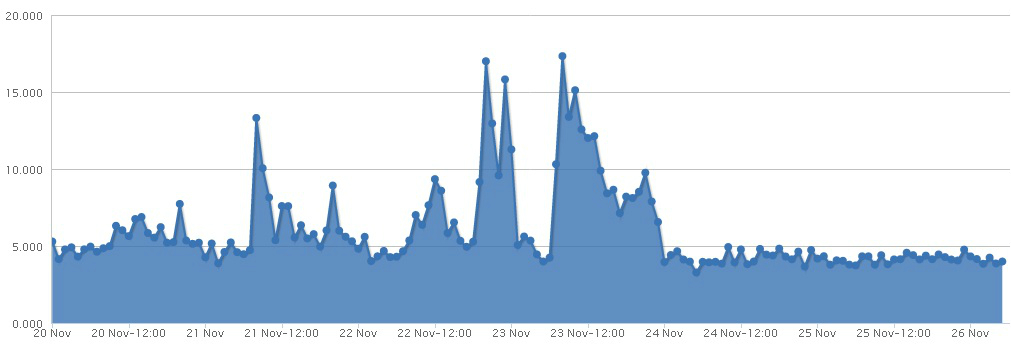
\includegraphics[scale=0.45]{grafico-black-friday.jpg}
	\caption{Tempo de resposta do \textit{Black Friday} Brasil 2012}
	\label{fig:grafico-black-friday}
	\fadaptada{blackfridayNews}
\end{figure}

As técnicas de gerenciamento de recursos são inúmeras, como as de inteligência artificial que utilizam lógica \textit{fuzzy}, algoritmos de mineração de dados e aprendizado de máquina \cite{Nobile2013}. As técnicas de aprendizado de máquina mostram-se interessantes para soluções imediatas, onde não há tempo hábil, inclusive, com abordagens não lineares empregadas para implementar um gerenciador de recursos responsável pela alteração dinâmica das capacidades computacionais. Outros trabalhos, como o \citeonline{Zhang2007}, buscam identificar padrões de comportamento na carga de trabalho e otimizar a provisão dinâmica dos recursos nas máquinas virtuais com base em algoritmos reativos. \citeonline{Quiroz2009} buscam detectar, por monitoramento, a padronização e a tendência da carga de trabalho com o objetivo de otimizar os recursos. \citeonline{Nobile2013} também propõe o uso de modelos de séries temporais para modelagem de tráfego de tempo real e previsão de demanda, que é usada para criar partições de conexões para diferentes classes de prioridade. \citeonline{Zhang2011}, utiliza de técnicas de estatística e avaliação dos recursos disponíveis para tomar a decisão de qual recurso deve ser alocado.

\citeonline{Dong2014} afirmam que atualmente a maioria das aplicações Web são concebidas com sistemas \textit{mult-tiers} (multi-camadas) devido à flexibilidade de escalabilidade.% O planejamento de capacidade é um passo importante para determinar a quantidade de recursos exigido para garantir determinada QoS. No entanto, em geral o planejamento de capacidade é basicamente uma decisão de longo prazo e quase estático, e os recursos são determinados pela taxa de utilização máxima da aplicação para evitar a pena excessiva de QoS.

\citeonline{Lourenco2015} afirmam que a partir de um planejamento de capacidade, e a gestão de recursos em tempo real aumenta a sofisticação da arquitetura da solução nos diversos níveis e complexidade, as abordagens convencionais para análise de sistemas computacionais modernos; e concluí que as dinâmicas emergentes das interligações desses sistemas \textit{mult-tiers} pode produzir efeitos transitórios sobre o desempenho, como resposta temporal, ou o amortecimento e/ou comportamento oscilatório. Uma vez que estes efeitos variáveis no tempo podem potencialmente afetar a capacidade de resposta, eficiência e até mesmo a estabilidade global, métodos e ferramentas para avaliação das propriedades dinâmicas de sistemas computacionais são de importância prática para fins da engenharia.

Há caso em que existe o interesse em controlar a dinâmica deste sistema, para tanto é necessário modelar o sistema em questão e projetar um controlador que manipulará a sua dinâmica. Para trabalhar com estes sistemas deve-se ser capaz de modelar a dinâmico do sistema, que em termos matemáticos é extrair um modelo matemático e analisar suas características dinâmicas. Um modelo matemático de um sistema dinâmico é definido como um conjunto de equações que representa a dinâmica de maneira relativamente razoável. Percebe-se que um modelo matemático não é exclusivo para um determinado sistema. Um sistema pode ser representando de muitas maneiras diferentes e, por conseguinte, podem ter diversos modelos matemáticos, dependendo da perspectiva, uns mais precisos que outros, e outros mais simplificados \cite{Ogata2001}.

Algumas vezes, é possível representar sistemas dinâmicos através de equações diferenciais obtidas com base nas leis básicas da física. Esses sistemas de equações diferenciais descrevem uma determinada dinâmica do sistema no domínio do tempo e, com o desenvolvimento dessas equações, é possível identificar propriedades fundamentais do sistema \cite{Nobile2013}. Quando a modelagem é muito dedutiva e muito complexa pode-se recorrer a métodos empíricos de identificação. Nesses, o modelo matemático é induzido mediante a comparação de entrada e saída.	

A avaliação por aferição, comparação de entrada e saída, medição direta via instrumentação apropriada adequa-se nesse caso; no entanto, é necessário a existência e disponibilidade do sistema ou protótipo, pois a avaliação é feita através de estímulos às entradas. A leitura de suas saídas, possibilita testes de caixa preta em que não são exigidos conhecimentos sobre o funcionamento interno do sistema \cite{Nobile2013}, como em um sistema dinâmico, no qual o comportamento do sistema evolui com o tempo, em resposta a estímulos externos.

\section{Motivação}

Embora amplamente aplicada e difundida em diversas áreas da engenharia e ciência, a avaliação de desempenho em regime transitório é pouco explorada e usada em sistemas computacionais, em função de que sistemas computacionais e suas aplicações não tem necessita dessa análise. O desenvolvimento, contudo, de sistemas distribuídos de larga escala e de alta complexidade altera essa realidade \cite{hpcs2015, Lourenco2015, medc}, devido ao comportamento dinâmico que não se apresenta nitidamente em avaliações estacionarias convencionais na computação. 

No \textit{\sigla{LaSDPC}{Laboratório de Sistemas Distribuídos e Programação Concorrente}}\footnote{\url{http://www.lasdpc.icmc.usp.br}}, onde desenvolve este projeto, trabalhos anteriores lidam com essa temática. O trabalho de \citeonline{Nobile2013}, um sistema com características dinâmicas, hospedado em um ambiente de computação em nuvem gerencia recursos elásticos por meio de mecanismos de provisão de QoS, técnicas de teoria de controle. Em outro trabalho, \citeonline{Lourenco2015} apresenta uma especificação de uma arquitetura conceitual que separa responsabilidades de simulação dinâmica em um conjunto de aspectos básicos, e formaliza um modelo de referência abstrata para a concepção de ferramentas de simulação. O trabalho de \citeonline{Edwin2015}, em desenvolvido também no LaSDPC, estuda e define uma metodologia de análise transiente dedicado a sistemas computacionais dinâmicos reais utilizando a especificação arquitetural proposto por \citeonline{Lourenco2015}. A principal contribuição pretendida é a formulação e definição de uma metodologia para seu emprego em sistemas, cuja a metodologia deverá ser capaz de descrever e especificar os passos para modelar o sistema, e analisar os resultados transiente mediante as variações na carga de trabalho. Para tanto, o trabalho de \citeonline{Edwin2015} utiliza de um \textit{benchmark} para a validação experimental de sua metodologia. No entanto, o \textit{benchmark} escolhido por \citeonline{Edwin2015}, Bench4Q, não contempla as especificações apresentadas por \citeonline{Lourenco2015}.

Segundo \citeonline{Binnig2009} os \textit{benchmarks} tradicionais não são suficientes para a análise desses novos serviços de elasticidade da Computação em Nuvem. O principal desafio dos novos \textit{benchmarks} são fazer com que as métricas ofereçam informações relevantes a esses diferentes serviços e com diferentes capacidades e garantias desses serviços. \citeonline{Dong2014} afirmam que, a maioria das aplicações Web são concebidas como sistemas de \textit{mult-tiers}, devido à flexibilidade e capacidade de reutilização de \textit{software}, porem é difícil de modelar o comportamento de aplicações Web de \textit{multi-tiers}, devido ao fato de que a carga de trabalho estimula a dinâmica do sistema nos diferentes níveis da camada.

No âmbito da análise de desempenho em sistemas computacionais, definimos o \textit{benchmarking} como o ato de medir e avaliar o desempenho computacional, protocolos de rede, dispositivos e redes, sob condições de referência, em relação a uma avaliação de referência. O objetivo deste processo de \textit{benchmarking} é permitir a comparação equitativa por diferentes soluções, ou entre desenvolvimentos subsequentes de um \textit{\sigla{SUT}{\textit{System Under Test}}}. \textit{Benchmarking} é o principal método para medir o desempenho de uma máquina ou sistema.

Apesar de existir diversos \textit{benchmarks} e ferramentas para o estudo, nenhuma delas estimulam a dinâmica do sistema e permite uma avaliação em regime transiente, que se faz necessário para a pesquisa de \citeonline{Edwin2015}. A proposta deste trabalho é modificar o \textit{benchmark} definido por \citeonline{Edwin2015} e adequá-lo de maneira em que estimule a dinâmica do sistema possibilitando uma avaliação transiente.


\section{Objetivo}
Este trabalho tem por objetivo a extensão do \textit{framework} de \textit{benchmark} Bench4Q afim de atender os requisitos do modelo \textit{\sigla{MEDC}{\textit{Monitor, Effector, Demanda and Capacity}}}, proposto por \citeonline{Lourenco2015}. O objetivo restringe-se ao módulo de modulação da carga de trabalho, gerado pelo \textit{benchmark}, acrescendo-o de provisões nativas para gerar perturbações capazes de excitar e produzir o regime transiente do sistema SUT do \textit{benchmark}, permitindo apreciar-se sua dinâmica. A contribuição almejada é a disponibilização de um \textit{benchmark} que auxilie a análise de sistemas dinâmico e que possibilite a analise transiente.



%==================== REVISAO 
\section{Revisão}
\subsection{MEDC}
\begin{frame}{Estudo de análise em regime transitório}
	\begin{itemize}
		\item \cite{Lourenco2015} discutem a abordagem de análise de estado estacionário vigente para avaliação de desempenho de sistemas computacionais
		
		\item apresenta um planejamento de experimentos de simulação destinados a análise transitória, especialmente em aplicações \textit{multi-tiers}.
	\end{itemize}
\end{frame}

\begin{frame}{Arquitetura conceitual MEDC}
	\begin{figure}
		\centering
		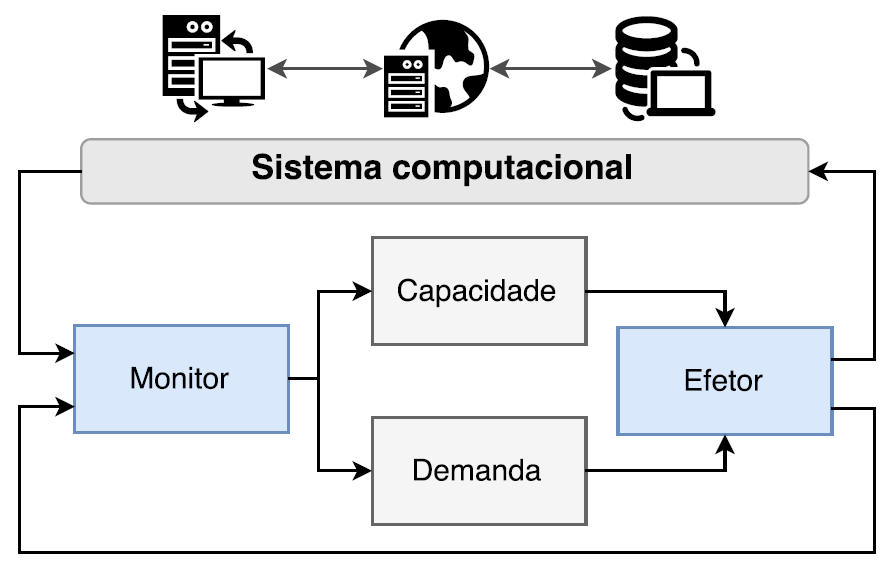
\includegraphics[scale=.4]{images/medc.png}
		\caption{MEDC: Monitor, Efetor, Demanda, Capacidade. \cite{Lourenco2015}}
		\label{fig:medc1}
	\end{figure}
\end{frame}

\begin{frame}{Modelo MEDC - o transiente}
	\begin{itemize}
		\item O transiente em um sistema computacional pode ser provocado por:
		\begin{itemize}
			\item Uma mudança na carga de trabalho 
			\item Uma mudança na capacidade interna (quantidade de recursos).
		\end{itemize}  
		\item O modelo MEDC mapeia esses dois aspectos nas responsabilidades respectivamente:
		\begin{itemize}
			\item \textbf{\textit{Demand} (modulação da carga)};
			\item \textit{Capacity} (modulação dos recursos).
		\end{itemize}
	\end{itemize}
\end{frame}



\begin{frame}{Modelo MEDC - demanda e capacidade}
	\note{no modelo MEDC diz que a ferramenta tem que incluir a pertubação de maneira programada realimentada (ex: quando a taxa de utilização ativem um nível)}
	\begin{itemize}
		%		\item O monitoramento produz as medidas para que a modulação de demanda e capacidade sejam feitas em tempo real;
		%		\begin{itemize}
		%			\item A saída do experimento deve produzir também gráficos temporais.
		%		\end{itemize}
		\item Uma perturbação pode ocorrer:
		\begin{itemize}
			\item Em função do tempo, (um acidente programado);
			\item Em função das medidas de desempenho, (de modo realimentado).
		
				\begin{itemize}
					\item \textbf{A modulação da carga} pode ser feita em função da \textit{taxa de requisições} (reduzir a carga admitida quando a utilização passar de certo limite).  
					\item \textbf{A modulação da capacidade} pode ser feita em função da utilização da CPU (aumentar os recursos quando a utilização ultrapassar certo patamar).  
				\end{itemize} 
		\end{itemize} 
	\end{itemize}
\end{frame}

%\begin{frame}{Modelo MEDC - Dinâmica}
%	\note{somente para completar o modelo, a capacidade e a demada dão os numeros mas quem atuaçõ é o Efector que é o mecanimos de atuação do Modelo}
%	\begin{itemize}
%		%		\item A modulação da demanda e a capacidade podem se refletir em: 
%		%		\begin{itemize}
%		%			\item política de admissão de carga;
%		%			\item gerenciamento de recursos.
%		%		\end{itemize} 
%		
%		\item A modelagem da dinâmica é responsabilidade do Efetor;
%		\begin{itemize}
%			\item O mecanismo pelo qual isso é implementado, fisicamente, pode \textbf{implicar em certa dinâmica}.
%			\item se a política de capacidade determina que os recursos devem ser aumentados, \textbf{o Efetor modela o atraso e a inércia} para a alocação e o desalocação dos recursos. 
%		\end{itemize}
%		
%	\end{itemize}
%\end{frame}



%\begin{frame}{O que é MEDC}
%	
%	\begin{columns}
%		\begin{column}{.4\textwidth}
%			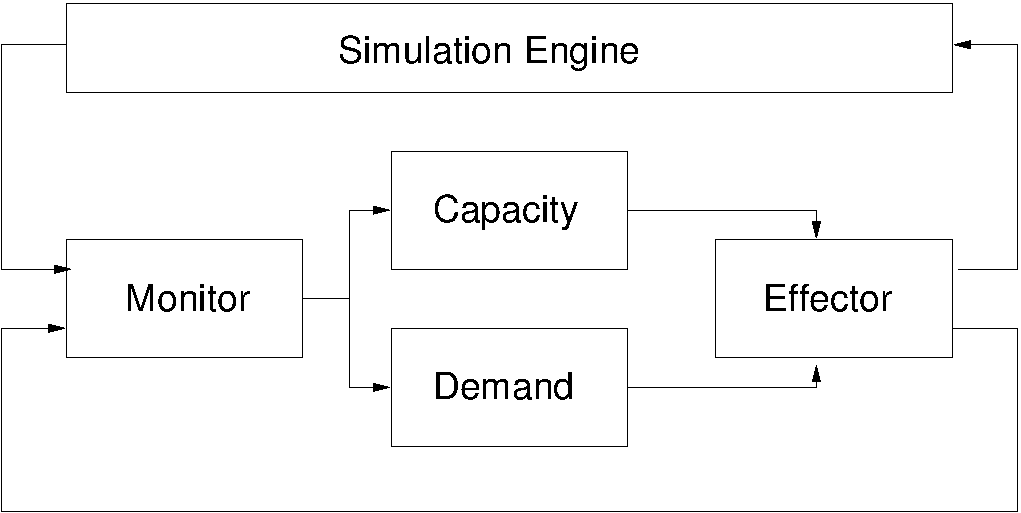
\includegraphics[width=.85\linewidth,valign=t]{../monograph/images/extension-block.pdf}
%
%		\end{column}
%		\begin{column}{.6\textwidth}
%			\textbf{"um conjunto de requisito que especificam uma arquitetura conceitual, intitulada MEDC (\textit{Monitor, Effector, Demanda and Capacity})."}
%			
%			\hfill-- Lourenço 2015
%		\end{column}
%	\end{columns}
%		
%	%\vspace*{10pt}
%	\begin{columns}
%		\begin{column}{0.9\textwidth}
%			\begin{itemize}
%				\item[\textit{Demand}:] referência para a capacidade de entrada e determinar a forma como a carga de trabalho muda ao longo do tempo;
%
%				\item[\textit{Capacity}:]  é a disposição análoga no que diz respeito aos recursos do sistema;
%				
%				\item[\textit{Monitor}:] sensor e aquisição de dados temporais, coletando os dados sobre o sistema e torná-lo disponível;
%				
%				\item[\textit{Effector}:] mecanismos de atuação através modulação, serve para a modelar os componentes operacionais que afetam a dinâmica \textit{Capacity} e \textit{Demand}.
%			\end{itemize}
%		\end{column}
%	\end{columns}
%\end{frame}



\subsection{Bench4Q}
%==================== BENCH4Q
\begin{frame}{Bench4Q}

\begin{itemize}
\item Bench4Q e um \textit{benchmark} para avaliação de desempenho em regime estacionário.

\item Não existem provisões para a introdução de perturbações programadas durante o experimento.

\item Código fonte disponível~\footnote{http://www.trustie.net/projects/project/show/Bench4Q}.

%\item Amplamente utilizado na literatura~\footnote{\cite{Wang2012b,Zhang2012a,Gao2013}}.

\item Fornece uma plataforma configurável e extensível para a execução de \textit{benchmarks}.
\end{itemize}


\end{frame}

\begin{frame}{Características}

Bench4Q:
\begin{itemize}
	\item É uma extensão do \textit{benchmark} \textbf{TPC-W} %\cite{Garcia2003}.
	\item Suporta analise de métricas baseadas em sessões.
	\item A geração de carga é baseada em agentes:
	\begin{itemize}
		\item Cada agente disponibiliza vários \textit{Workers} ou EBs (\textit{Emulate Browsers}).
		\item Agentes locais ou remotos.
	\end{itemize}
	\item Utiliza uma loja de livros: \textit{System Under Test} (\textbf{SUT}).
	\begin{itemize}
		\item Simula um sistema \textit{e-commerce}, multicamada (Web e banco de dados);
	\end{itemize}
\end{itemize}

\end{frame}

\begin{frame}{Caraterísticas}
	\begin{figure}
		\begin{center}
			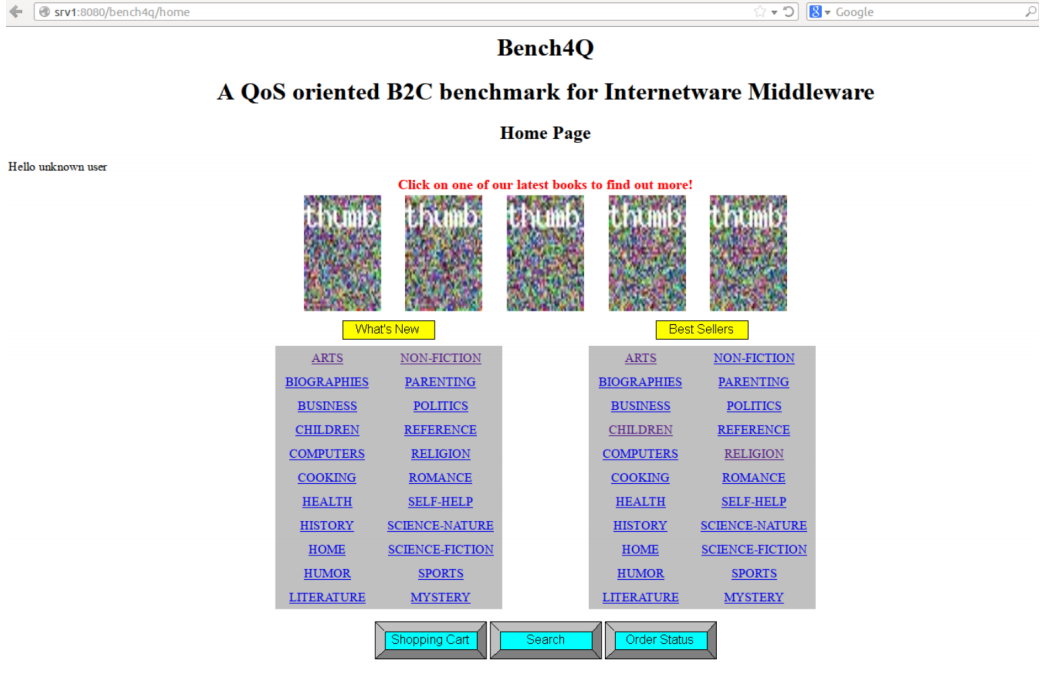
\includegraphics[scale=0.35]{images/sut.png}
			\caption{Bench4Q: SUT.}
			\label{fig:sut-bench4q}
		\end{center}
	\end{figure}
\end{frame}


\begin{frame}{Métricas disponíveis no Bench4Q}
%Métricas de interesse disponíveis no Bench4Q:
\begin{itemize}
	\item WIRT (\textit{Web Interaction Response Time}) - TPC-W
	\item WIPS (\textit{Web Interacton Per Second}) - TPC-W
	\item VSPS (\textit{Valid Sessions Per Second}) - Bench4Q
	\item VSR (\textit{Valid Sessions Ratio}) - Bench4Q	
\end{itemize}

\end{frame}

\begin{frame}{Métricas disponíveis no Bench4Q}
\begin{figure}
	\begin{center}
		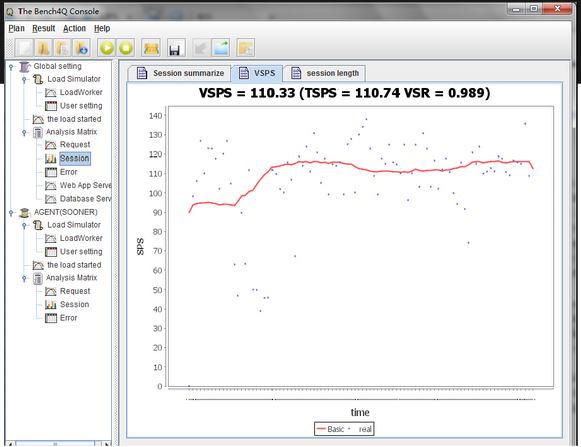
\includegraphics[scale=0.5]{images/metricas.png}
			\caption{Bench4Q: Métrica VSPS.}
					\label{fig:vsps-bench4q}
	\end{center}
\end{figure}

\end{frame}

\begin{frame}{Arquitetura Bench4Q}
	\begin{figure}
		\begin{center}
			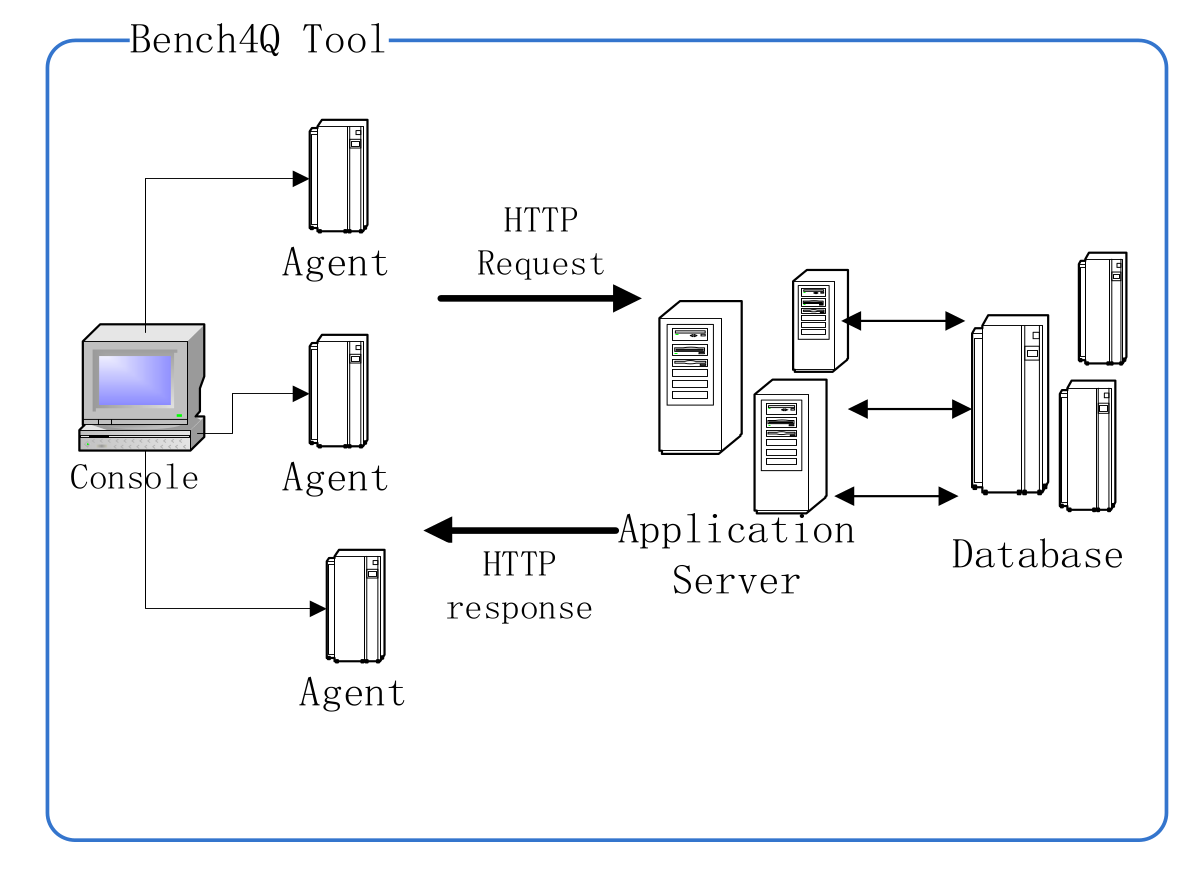
\includegraphics[scale=0.2]{images/bench4Q.png}
			\caption{Arquitetura Bench4Q \cite{Bench4Q}.}
			\label{fig:arquitetura-bench4q}
		\end{center}
	\end{figure}
\end{frame}

\begin{frame}{Gerador de carga}
  \putat{120}{-100,5}{
  	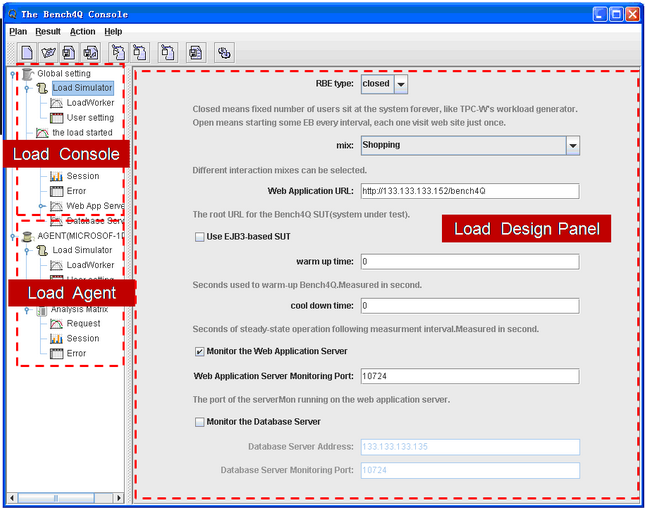
\includegraphics[scale=0.4]{images/console-bench4Q.png}
  }
\begin{itemize}
\item Tipos de carga:
\begin{enumerate}
	\item \textit{Browsing}
	\item \textit{Ordering}
	\item \textit{Shopping}
\end{enumerate}
%\item Gerenciamento dos agentes.
\end{itemize}  


\end{frame}

\begin{frame}{Comportamento dos EBs}
CBMG (\textit{Customer Behavior Model Graph}) é um grafo estatístico que modela o comportamento de navegação de um usuário(emulado).

	\begin{figure}
		\center
		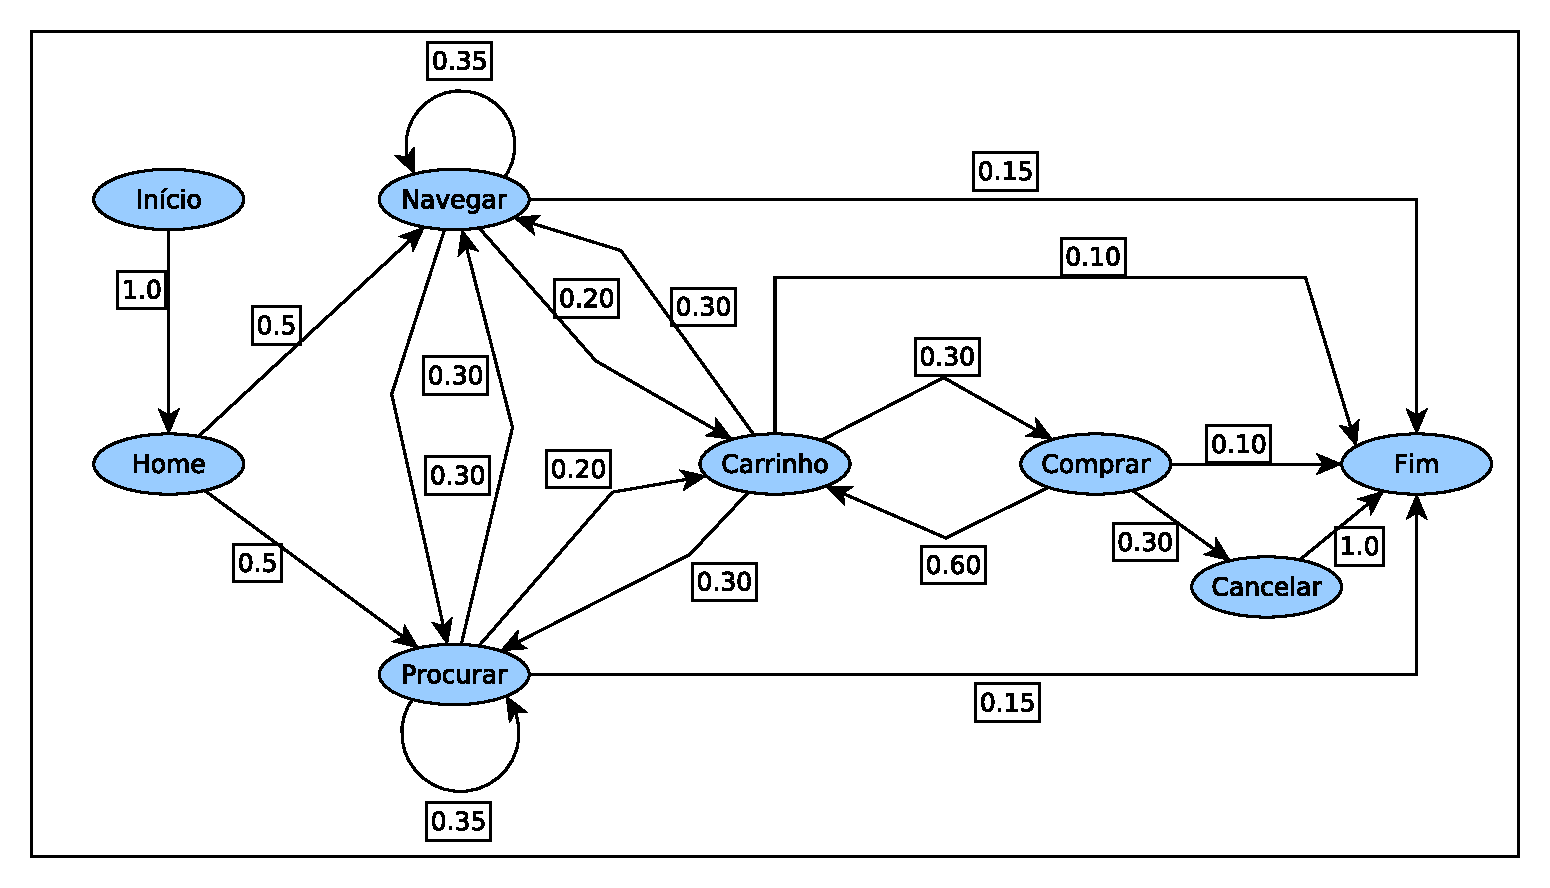
\includegraphics[scale=0.35]{images/CBMG}
		\caption{Perfil interação estocástico com o sistema (SUT).}
		\label{fig:CBMG}
	\end{figure}
\end{frame}



%==================== Metodologia
\section{Metodologia}
\begin{frame}{Parâmetros para moduladar a carga}
	\begin{itemize}
		\item \textbf{Tempo de planejamento de carga:} Um período de tempo em que a carga de trabalho é modulada, caracterizando a mudança do comportamento das requisições de maneira programada;
		
		\item \textbf{Tipo de modulação:} a modulação será apresentada conforme as funções ou sinais propostos por \cite{Hellerstein2004};
		
		\item \textbf{Tempo de interrupções:} Período de interrupções/pausa após o \textit{Tempo de planejamento de carga};
		
		\item \textbf{Quantidade de clientes na modulação:} reservar uma quantidade de clientes EBs, que estão com dedicação exclusiva para a modulação da carga.
	\end{itemize}	
\end{frame}

\begin{frame}{Possibilidade de cargas moduláveis pela extensão}
	\begin{columns}
		\column{0.5\textwidth}
		\begin{minipage}[c][0.4\textheight][c]{\linewidth}
			\centering
			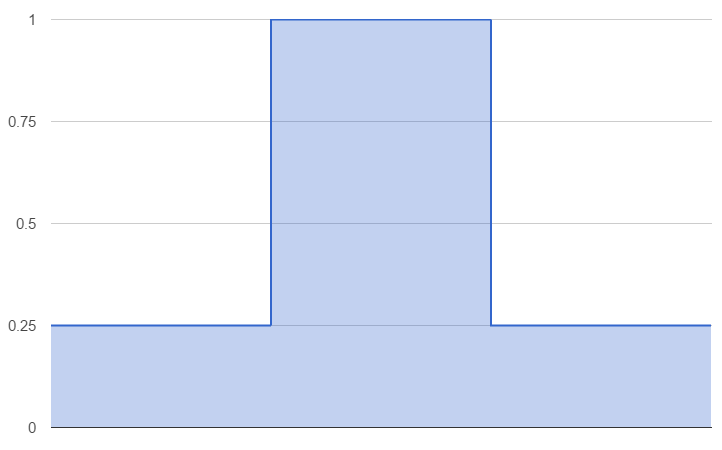
\includegraphics[width=0.8\linewidth]{../monograph/images/carga-sintetica1.png}
			\label{fig:degrau-positivo}
		\end{minipage}
		\begin{minipage}[c][0.4\textheight][c]{\linewidth}
			\centering
			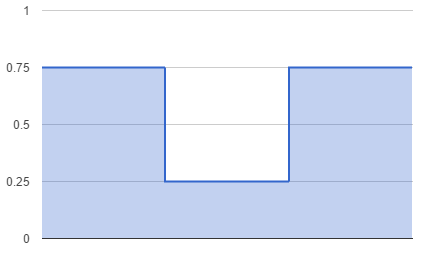
\includegraphics[width=0.8\linewidth]{../monograph/images/carga-sintetica2.png}
			\label{fig:degrau-negativo}
		\end{minipage}
		\column{0.5\textwidth}
		\begin{minipage}[c][0.4\textheight][c]{\linewidth}
			\begin{enumerate}
				\item Degrau positivo,
				\item Degrau negativo,
				\item Onda quadrada;
			\end{enumerate}
		\end{minipage}
		\begin{minipage}[c][0.4\textheight][c]{\linewidth}
			\centering
			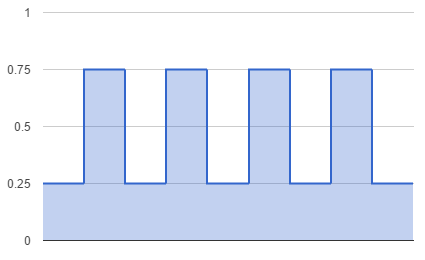
\includegraphics[width=0.8\linewidth]{../monograph/images/carga-sintetica3.png}
			\label{fig:onda-gradrada}
		\end{minipage}
	\end{columns}
\end{frame}

\begin{frame}{Arquitetura do experimento}
	\begin{columns}
		\column{0.4\textwidth}
		\begin{minipage}[c][0.4\textheight][c]{\linewidth}
			\centering
			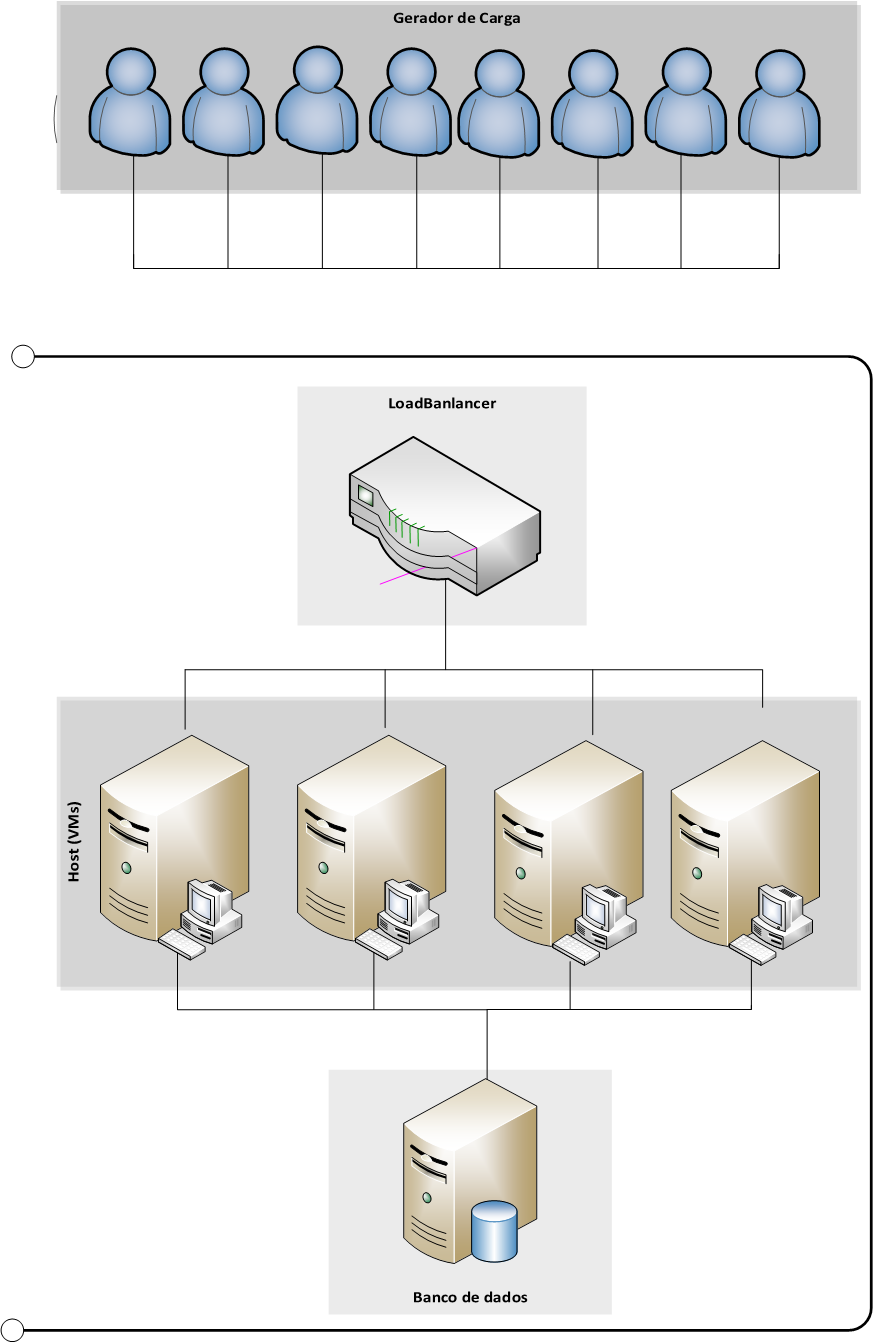
\includegraphics[scale=0.17]{../monograph/images/arquitetura-experimento.png}
			\label{fig:arquitetura-experimento}		
		\end{minipage}
		\column{0.6\textwidth}
		\begin{minipage}[c][0.4\textheight][c]{\linewidth}
			\begin{itemize}
				\item Gerador de Carga (\textit{Workload})
				\item Balanceador de carga (\textit{Load Balancer})
				\item Servidor Físico (\textit{Hypervisor})
				\item Servidor de dados (\textit{Data base})
			\end{itemize}
		\end{minipage}		
	\end{columns}
	
\end{frame}

\begin{frame}{Comportamento de métrica transiente}

\end{frame}

\begin{frame}{Comportamento de métrica transiente}
	\begin{columns}
		\column{0.45\textwidth}
		\begin{minipage}[c][0.45\textheight][c]{\linewidth}
			\centering
			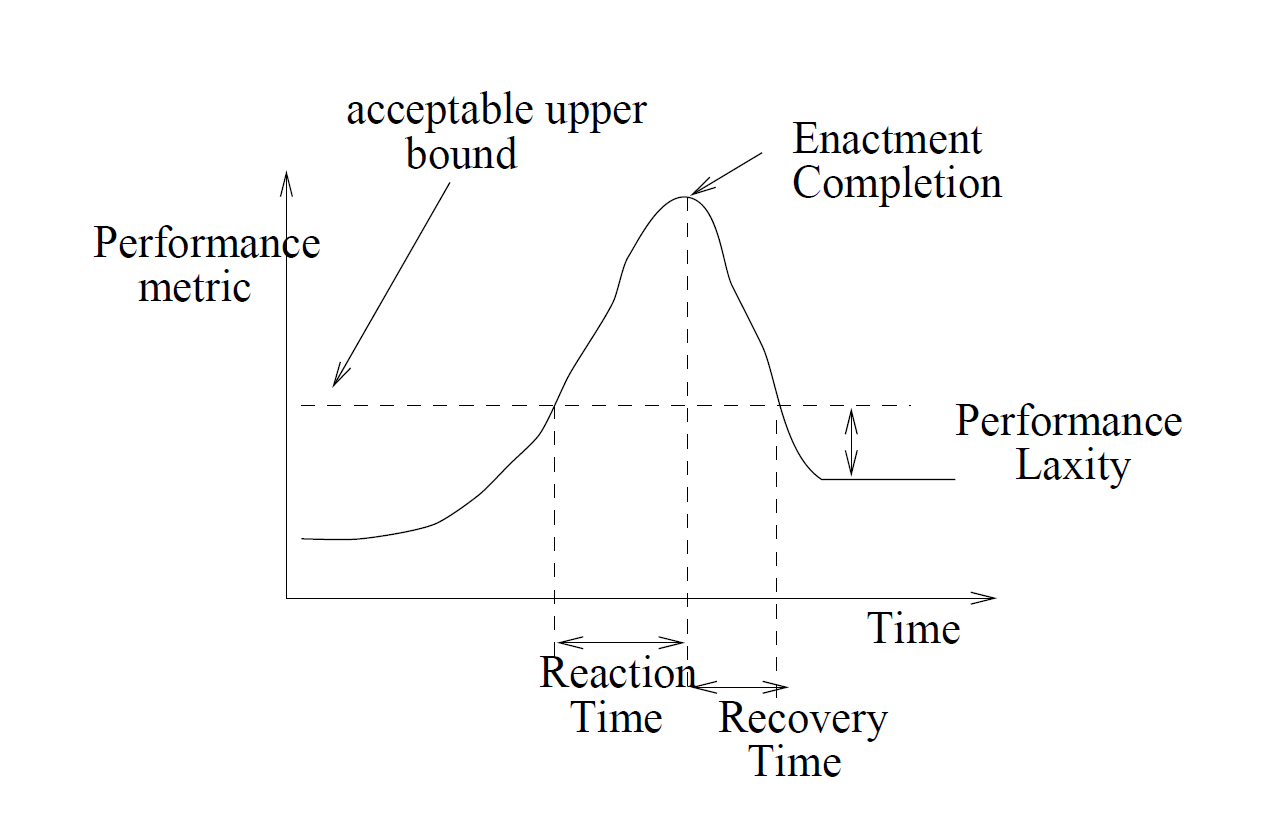
\includegraphics[width=1.27\linewidth]{../monograph/images/transient-metric.png}
			\label{fig:transient-metric}	
		\end{minipage}
		\column{0.55\textwidth}
		\begin{minipage}[c][0.55\textheight][c]{\linewidth}
			\begin{itemize}
				\item \textbf{\textit{Reaction Time} (Tempo de reação)} - o período entre a ocorrência da variação crítica e a conclusão da promulgação realocação de correção;
				
				\item \textbf{\textit{Recovery Time} (Tempo de Recuperação)} - o intervalo entre a conclusão, promulgação e da restauração de um nível de desempenho aceitável;
				
				\item \textbf{\textit{Performance Laxity} (Frouxidão performance)} - a diferença entre o \textit{required vs performance}, e o desempenho em estado estacionário, após a redistribuição;
			\end{itemize}
		\end{minipage}		
	\end{columns}
\end{frame}

\begin{frame}{Métrica transiente}
	\begin{itemize}
		\item \textbf{Conexões por segundo (\textit{Load Balancer}):} Conforme sugerido por \cite{Binnig2009}, medir a escalabilidade através do aumento dos interações web emitidos por segundo ao longo do tempo e de forma contínua contando a interação web que são respondidas em um intervalo de tempo de resposta,
		
		\item \textbf{Tempo de resposta (\textit{browsers}):} \cite{helder2014}, em um sistema dinâmico, cuja transformação entrada-saída não ocorre em tempo zero, mas é sujeita a uma inércia advinda dos processos físicos associados, possuí uma inércia intrínseca que atrasa o efeito que uma entrada terá na saída. Esses efeitos refletem no consequentemente nos comportamentos diversos que incluem retardo no tempo de resposta e possíveis oscilações; 	
	
	\end{itemize}
\end{frame}

\begin{frame}{Métrica transiente}
	\begin{itemize}
		\item \textbf{Taxa de utilização da CPU (VMs):} \cite{Nobile2013} afirma que diversas métricas podem ser analisadas para verificar o desempenho das máquinas virtuais, e cita alguns exemplos, como o tempo de inicialização, a taxa de utilização de CPU, o tempo médio de resposta e o \textit{throughput}, e usualmente, número de máquinas virtuais que hospedam serviços de interesse ao cliente e que respondem a uma carga de trabalho imposta por usuários através de requisições;
		
		\item \textbf{Taxa de utilização da CPU:} O trabalho apresentado por \cite{wang2009}, que lida com uma carga de trabalho variante no tempo e intensiva, demonstra que a CPU e I/O podem ser utilizadas para prever as necessidades dos recursos de um banco de dados e para orientar a alocação de recursos \textit{on-demand} de acordo com a exigência de carga de trabalho. Entretanto iremos somente considerar em nossos experimento a taxa de utilização do banco de dados.
	\end{itemize}
\end{frame}

\begin{frame}
	PEGAR IMAGEM DO EDWIN QUE EXPLICA A RESERVAR DOS EBs
\end{frame}



%==================== Desenvolvimento
\section{Desenvolvimento}
Nesta seção é apresentado em detalhes a implementação aplicada no \textit{benchmark} Bench4Q. A Figura \ref{fig:diagrama-classes} mostra o diagrama de classes envolvido na extensão do Bench4Q. As classes sinalizadas na cor azul, representam as já existentes mas que passaram por adaptações e modificações, já as classes na cor verde, referem-se as novas classes criadas para possibilitar a modulação da carga do \textit{benchmark}.

Apesar de permitir a geração de carga para o sistema, o Bench4Q possui algumas limitações na sua versão original que dificultam a experimentação e analise de cenários de interesse ao trabalho de \citeonline{Edwin2015} e \citeonline{Lourenco2015} de quem pretende desenvolver técnicas de gerenciamento de recursos.
As classes disponíveis no \textit{benchmark} original não permitem a modulação de carga de trabalho, essa limitação implica, por exemplo, na dificuldade de projetar um controlador para o gerenciamento de recursos, pois para esta atividade é necessário uma análise de resultados transientes mediante a modulação da carga de trabalho. A simulação de uma carga de trabalho em que há a alteração introduzida ao longo da simulação é o foco deste trabalho.

\begin{figure}[!htb]
	\centering
	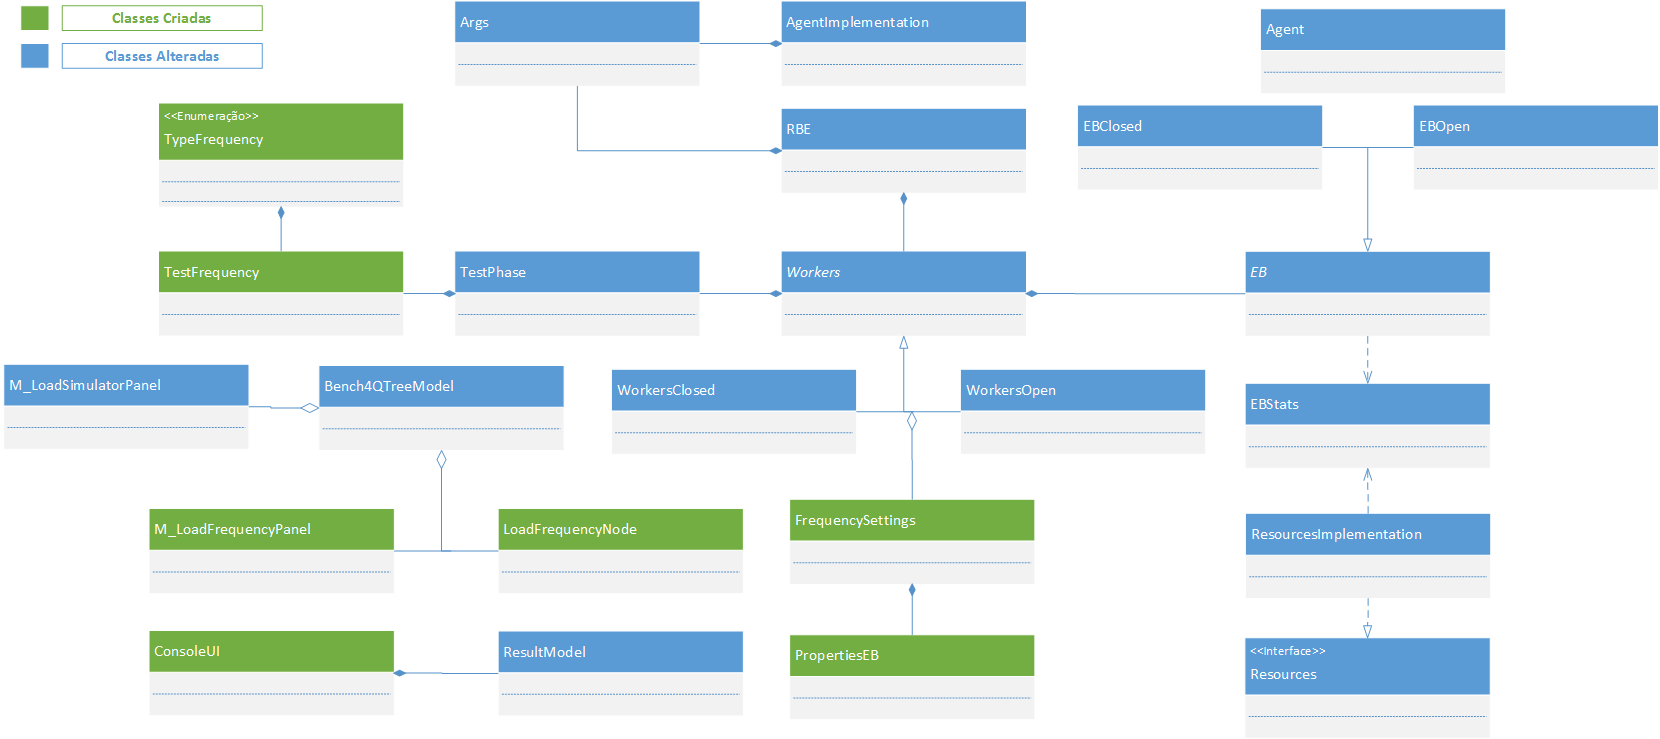
\includegraphics[angle=90, scale=0.6]{diagrama-classes-beanch4Q.png}	
	\caption{Diagrama de classes da extensão do Bench4Q.}
	\label{fig:diagrama-classes}
	\fautor
\end{figure}

Para distribuir a submissão da carga de trabalho ao longo da simulação, uma estratégia utilizada é a modulação da mesma através de parâmetros que configuram o comportamento da carga. O Bench4Q também não suporta nativamente a alocação e a deslocação dos recursos em tempo de simulação, uma conjunto de implementações foram necessárias para estender o \textit{benchmark}, essas aplicações não lidam com a modulação da carga de trabalho, mas manipulação a distribuição da carga de trabalho em um conjunto de servidores, da mesma maneira que um ambiente de nuvem, assim como o gerenciamento dos recursos da proposta de arquitetura. Contudo, os detalhes dessa implementação não serão apresentados e discutidos neste trabalho, uma vez este contexto foge do foco e da proposta do trabalho que tem por objetivo a modulação da carga.



%1º  - falar como foi implementados as modificações conforme a metodologia

A princípio foi identificado o modulo de geração de carga do Bench4Q e este passou por alterações para gerar a carga de trabalho esperada. Conforme o diagrama de classes na Figura \ref{fig:diagrama-classes}, é possível ter uma ideia do trabalho de extensão realizado no \textit{benchmark}, vale aqui salientar que o Bench4Q é uma ferramenta completa e extensa, e diagramar todas as classes do mesmo ficaria difícil e aumentaria consideravelmente a complexidade de entendimento, sendo assim, aqui apresentamos somente as classes já existem no Bench4Q e que passaram por modificações para atender aos requisitos da proposta, juntamente com as novas classes que foram necessárias para almejar o mesmo objetivo.

O Bench4Q fornece uma estrutura e componentes compartilhados para a comunicação entre os dois módulos da carga de trabalho, \textbf{Console} e \textbf{Agente}. Apesar de trabalharem em conjunto e para um mesmo fim, cada modulo (Console e Agente) é executado em máquinas distintas.  A extensão é construída inicialmente sob a classe \textsf{MLoadSimulatorPanel}, que orquestra toda a interatividade gráfica do Bench4Q. O novo painel de configuração, que modula a carga, \textsf{MLoadFrequencyPanel} estende da classe original \textsf{Bench4QTreeModel}, adicionando os parâmetros para a modulação: tipo da carga, o instante em que a carga se inicia, o tempo de atuação da carga e a quantidade de EBs que atuaram nessa carga. O parâmetro \textit{"tipos de carga"}, utiliza da classe enum \textsf{TypeFrequency} que define as constantes dos tipos de modulações programadas para esta extensão.  Todos os parâmetros inseridos na \textsf{MLoadSimulatorPanel} são armazenados na classe \textsf{TestFrequency} que se tornou uma propriedade da classe nativa \textsf{TestPhase}, que posteriormente são repassadas para a classe \textsf{PropertiesEB} através da \textsf{FrequencySettings}. Já nas classes \textsf{Agent}, \textsf{EB}, \textsf{EBClose}, \textsf{EBOpen}, \textsf{Workers}, \textsf{WorkersClosed} e \textsf{WorkersOpen} foram modificadas para receber os novos parâmetros da \textsf{PropertiesEB} e compreendê-los correspondentemente a modulação configurada na interface gráfica e gerando a carga programada durante a execução.

O código-fonte \ref{code:modelworkload}, é um pseudo-código que ilustra o esqueleto de maneira simplificada do \textit{core} da geração da carga referente a construção da modulação da carga já com as modificações da extensão.

\begin{codigo}[caption={Algoritmo de geração de carga modificado para modulaçao}, label={code:modelworkload}, breaklines=false]
ParametrosExperimento parametros;
	
ebCorrente.EmExecucao = true;
while (parametros.ExperimentoEmExecucao) {
		
	tempoCorrente = System.pegaTempoCorrente();
	
	if (tempoCorrente > parametros.TempoExperimento){
		ebCorrente.EmExecucao = false;
	}
	
	if (tempoCorrente > ebCorrente.TempoDuracao && ebCorrente.EbMarcado) {
		if(parametros.TempoPausa > 0){
			
			long novoInicio = ebCorrente.TempoFinal + parametros.TempoPausa ;
			long periodo = ebCorrente.TempoFinal - ebCorrente.TempoInicial;
			
			ebCorrente.TempoInicial = novoInicio;
			ebCorrente.TempoFinal = periodo + novoInicio;
		} else if (tempoCorrente > ebCorrente.TempoInicial) {
			ebCorrente.EmExecucao = false;
		}
	}

	if (tempoCorrente >= ebCorrente.TempoInicio) {
		if (!ebCorrente.EmExecucao) {
			return;
		}
		if (ebCorrente.TemProximaPagina) {
			// fluxo de acesso a pagina do SUT (recurso nativo do Bench4Q)
		} else {
			ebCorrente.EmExecucao = false;
		}	
		if (!ebCorrente.EmExecucao = false;) {
			return;
		}	
	} else {
		ebCorrente.Dorme(500);				
	}

}

\end{codigo}


Este conjunto de classes as quais lidam, manipulam, gerenciam e modulam a carga de trabalho gerada pelo Bench4Q, utilizam de um excelente console para configurar, monitorar e analisar todo o experimento. Todo o desenvolvimento, referente à modificação e implementação de novas classes, mantiveram e respeitaram o padrão de desenvolvimento do \textit{benchmark}. A Figura \ref{fig:interface-criada-beanch4q} ilustra a interface gráfica por onde é possível modular a carga de trabalho do Bench4Q. 


No console principal do Bench4Q, onde configura a execução do experimento, foi incluído uma nova opção \textit{LoadFrequency} referente ao parâmetros da extensão da geração da carga modulada. Por esta opção, \textit{LoadFrequency}, deve-se preencher os campos (\textit{Start Time}, \textit{Duration Step}, \textit{Pause} e \textit{Quantity}) que irão gerar a carga modulada conforme a programação. A característica de todos os resultados de desempenho de cada agente de carga são agregados para o console de carga para análise e demonstração, mantem-se conforme a versão original.
Informar previamente a execução os parâmetros da modulação, como por exemplo, ao escolher a opção degrau, é necessário informar quantos EBs geram o degrau, em que instante de tempo, e qual o tempo de duração e por fim qual a sua polaridade (com base em um pulso elétrico a positiva sairia de zero e chega a um, a negativa, sairia de um e chegaria a zero), é possível obter resultados conforme a Figura \ref{fig:grafico-carga-modulada-teste}.

\begin{figure}[!htb]
	\centering
	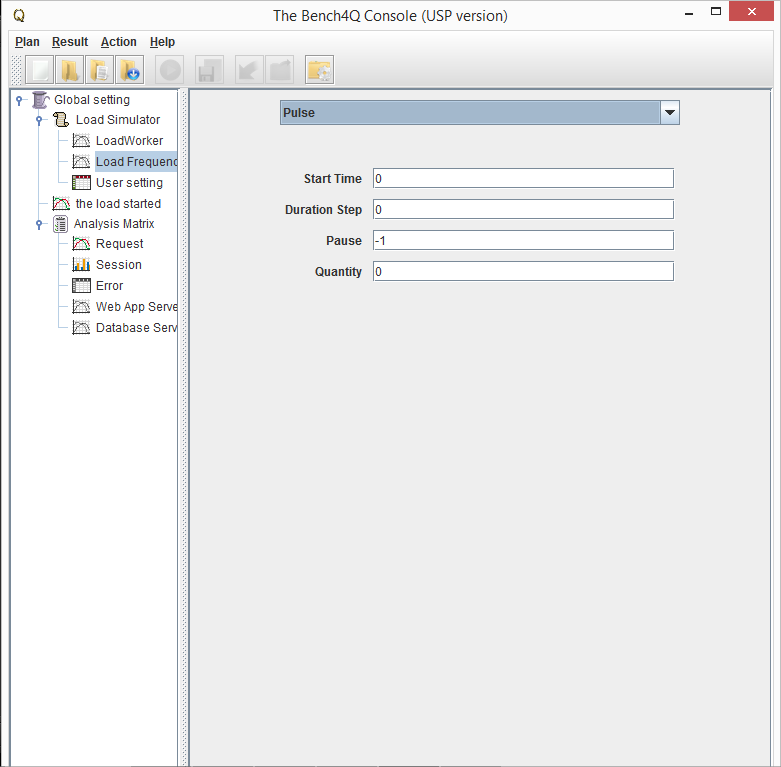
\includegraphics[scale=0.6]{console-bench4Q-usp.png}
	\caption{Console de programação de carga de trabalho.}
	\label{fig:interface-criada-beanch4q}
	\fautor
\end{figure}

A carga de trabalho é imposta ao sistema por meio de requisições HTTP enviadas pelos EBs ao SUT que são executadas nos servidores de aplicação das máquinas virtuais instanciadas no \textit{host}. Essas requisições exigem que as máquinas virtuais se ocupem pelo tempo necessário para processá-las, alterando o desempenho experimentado pelo sistema.
Segundo \citeonline{Nobile2013}, existem dois fatores que envolvem uma requisição e que afetam diretamente o desempenho do sistema:
\begin{citacao}
	o tempo de processamento e a quantidade de carga imposta pelas requisições, são dados pelo tempo de processamento e pela taxa de chegada de novas requisições, respectivamente. Com o tempo, a quantidade e o tamanho das requisições podem se alterar, dependendo do perfil de utilização dos usuários que utilizam o serviço naquele momento. Havendo um aumento em algum desses fatores é possível que o desempenho do sistema sofra degradação, podendo, em casos extremos, entrar em colapso.
\end{citacao}

\begin{figure}[!htb]
	\centering
	\begin{subfigure}{\linewidth}
		\centering
		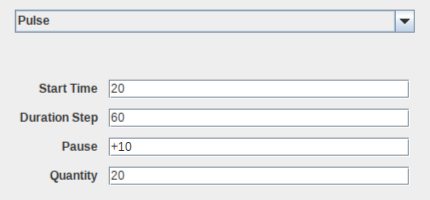
\includegraphics[scale=0.7]{condiguracao-carga-modulada1.png}
		\caption{Teste de configuração da carga a ser modulada}
		\label{fig:configuracao-carga-modulada-teste}
	\end{subfigure}
	
	\begin{subfigure}{\linewidth}
		\centering
		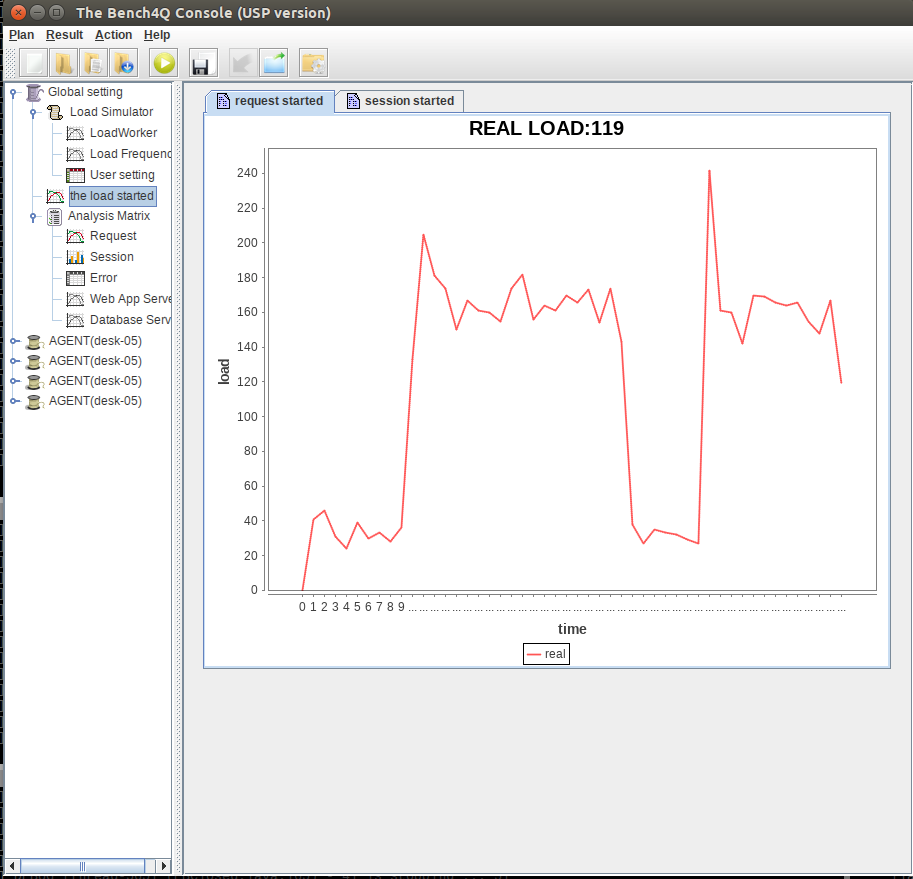
\includegraphics[scale=0.6]{grafico-carga-modulada-teste.png}
		\caption{Carga gerada com base na configuração teste}
		\label{fig:grafico-carga-modulada-teste}
	\end{subfigure}  
	\caption{Teste de modulação da carga}  
	\label{fig:carga-modulada-teste}
	\fautor
\end{figure}  

A Figura \ref{fig:carga-modulada-teste} ilustra uma carga teste modulado já pela extensão, na Figura \ref{fig:configuracao-carga-modulada-teste} apresenta os parâmetros utilizado para fazer o teste, a carga modulada atuará a partir do 10º segundo de experimentação e com uma duração de 20 segundos, com 30 segundos de experimentação ocorrerá uma pausa de 7 segundos e um novo degrau será gerado em seguida, que se manterá até o final do experimento. Para este exemplo foram fixados 40 EBs para modularizar o comportamento da carga. Este comportamento pode ser apreciado no item \ref{fig:grafico-carga-modulada-teste} da mesma figura \ref{fig:carga-modulada-teste}. Vale salientar que o gráfico gerado e apresentado na figura \ref{fig:carga-modulada-teste} de item \ref{fig:grafico-carga-modulada-teste}, é uma característica nativa ao \textit{benchmark}.

O Bench4Q, possui uma documentação sobre a ferramenta. Devido a extensão do \textit{benchmark} foi elaborada uma documentação seguindo os padrões da última versão original e esta pode ser conferida no apêndice A que traz informações do programa e qual seu objetivo, entradas suportadas e saídas esperadas, exemplo de como executar o programa e tabela descrevendo as principais características do mesmo.

%==================== Resultados
\section{Resultados}
As análises apresentadas nessa seção resume os resultados dos testes exemplares na extensão feita no Bench4Q, os resultados aqui mostrados são proporcionados como exemplos de aplicação da metodologia, eles não devem ser interpretados como definitivos e avaliações de desempenho. Dessa forma, para uma melhor abordagem dos exemplos apresentados, os exemplo divide-se em 3 partes:
\begin{itemize}
	\item Configuração da carga no Bench4Q
	\item Configuração para modular a carga
	\item Carga gerada
\end{itemize}

\begin{figure}[!htb]
	\begin{subfigure}{\linewidth}
		\centering
		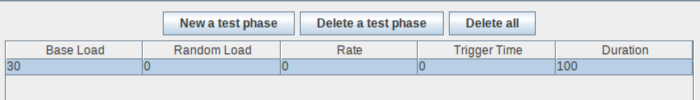
\includegraphics[scale=0.7]{condiguracao-carga-bench4q1.png}
		\caption{Configuração da carga no Bench4Q, para um degrau positivo}
		\label{fig:condiguracao-carga-bench4q1}
	\end{subfigure}\\
	\begin{subfigure}{\linewidth}
		\centering
		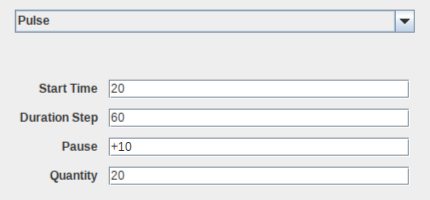
\includegraphics[scale=0.7]{condiguracao-carga-modulada1.png}
		\caption{Configuração para modular a carga como um degrau positivo}
		\label{fig:condiguracao-carga-modulada1}
	\end{subfigure}\\[1ex]
	\begin{subfigure}{\linewidth}
		\centering
		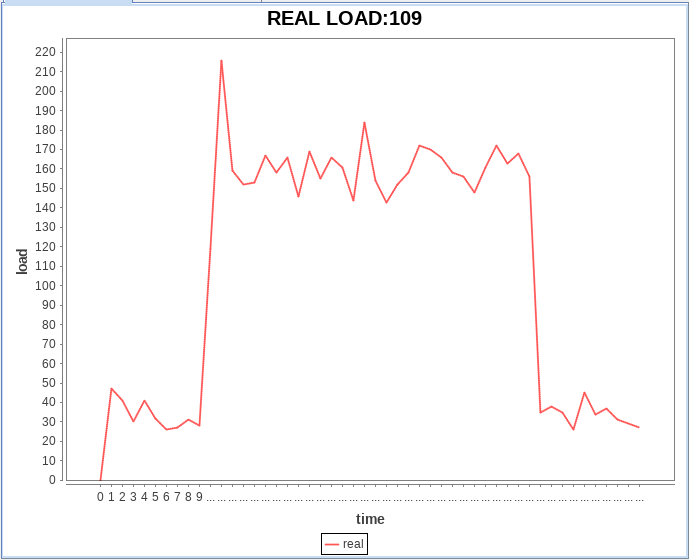
\includegraphics[scale=0.6]{grafico-carga-modulada1.png}
		\caption{Carga gerada com base nas configuração}
		\label{fig:grafico-carga-modulada1}
	\end{subfigure}
	\caption{Carga gerada com base na configuração: Degrau Positivo}
	\label{fig:carga-modulada1}
	\fautor
\end{figure}

A figura \ref{fig:carga-modulada1} apresenta a primeira exemplificação gerada com o Bench4Q já com a extensão desenvolvida neste trabalho, na figura \ref{fig:condiguracao-carga-bench4q1} demonstra os parâmetros de configuração utilizados para gerar a carga, dois são os principiais, \textit{Base Load} e \textit{Duration}, o primeiro define a quantidade e EBs envolvidos nos experimento, neste caso 30 EBs, já o segundo define o tempo de duração do experimento em segundos, neste caso 100 segundos. Na figura \ref{fig:condiguracao-carga-modulada1} são apresentados os parâmetros para modular a carga \textit{Start Time} de valor 20, refere-se ao tempo de esperara para o inicio do restante da carga se mostrar presente e ativa na modulação, assim decorrido 20 segundos os 20, dos 30 EBs, definido pelo \textit{Quantity} iniciam a gerar carga para o sistema, essa carga se manterá ativa durante 60 segundos conforme fixado no parâmetro \textit{Duration Step}, neste exemplo o parâmetro \textit{Pause} não apresentar influencia devido ao seu valor 0.
O resultado pode ser apreciado pela figura \ref{fig:grafico-carga-modulada1}, este gráfico é nativo do próprio Bench4Q, que demonstra o comportamento da carga no decorrer do tempo. Apesar da estocasticidade a carga se modulou conforme programada, essa estocasticidade é característica do Bench4Q, afim de manter um comportamento mais realístico com os de clientes acessando uma estocasticidade \textit{E-commerce}.

\begin{figure}[!htb]
	\begin{subfigure}{\linewidth}
		\centering
		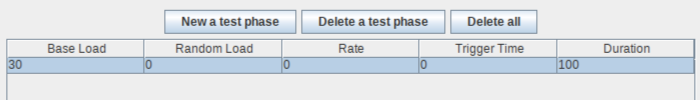
\includegraphics[scale=0.7]{condiguracao-carga-bench4q2.png}
		\caption{Configuração da carga no Bench4Q, para um degrau negativo}
		\label{fig:condiguracao-carga-bench4q2}
	\end{subfigure}\\
	\begin{subfigure}{\linewidth}
		\centering
		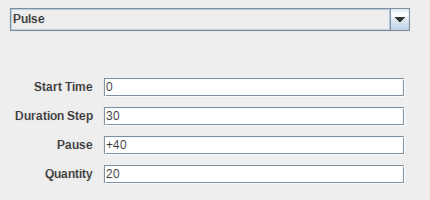
\includegraphics[scale=0.7]{condiguracao-carga-modulada2.png}
		\caption{Configuração para modular a carga como um degrau negativo}
		\label{fig:condiguracao-carga-modulada2}
	\end{subfigure}\\[1ex]
	\begin{subfigure}{\linewidth}
		\centering
		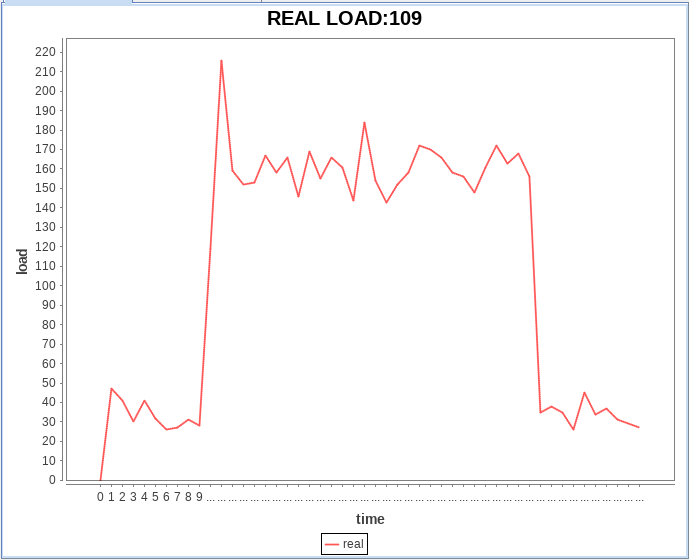
\includegraphics[scale=0.6]{grafico-carga-modulada2.png}
		\caption{Carga gerada com base nas configuração}
		\label{fig:grafico-carga-modulada2}
	\end{subfigure}
	\caption{Carga gerada com base na configuração: Degrau Negativo}
	\label{fig:carga-modulada2}
	\fautor
\end{figure}

A figura \ref{fig:carga-modulada2} apresenta os resultados dos parâmetros para o objetivo do Degrau Negativo. Os parâmetros de \textit{Base Load} e \textit{Duration} são os mesmos do experimento anterior, 30 EBs e 100 segundos de execução, conforme apresentado na figura \ref{fig:condiguracao-carga-bench4q2}. Já na \ref{fig:condiguracao-carga-modulada3} que demonstra os parâmetros utilizados para modular a carga, o \textit{Start Time} recebe o valor 0, assim a carga modulado iniciar com potência máxima utilizando os 30 EBs sendo 20 EBs setado no \textit{Quantity} para reservá-los para a modulação, o tempo de carga máxima é de 30 segundos como é possível ver no parâmetro \textit{Duration Step}, neste caso o \textit{Pause} é setado com 40 segundos, este valor é o que fará a interrupção brusca dos 20 EBs caindo o nível da geração de carga, gerando o degrau negativo. Passado esse período de pausa, a carga retorna ao seu nível máxima e atua por mais 30 segundos, o resultado final pode ser visto na figura \ref{fig:grafico-carga-modulada2}. 
%vale chamar a atenção para a dinâmica apresentada pela geração da carga sempre ao atingir o nivel maximo

\begin{figure}[!htb]
	\begin{subfigure}{\linewidth}
		\centering
		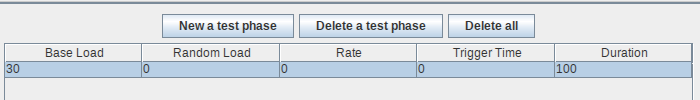
\includegraphics[scale=0.7]{condiguracao-carga-bench4q3.png}
		\caption{Configuração da carga no Bench4Q, para uma onda quadrada}
		\label{fig:condiguracao-carga-bench4q3}
	\end{subfigure}\\
	\begin{subfigure}{\linewidth}
		\centering
		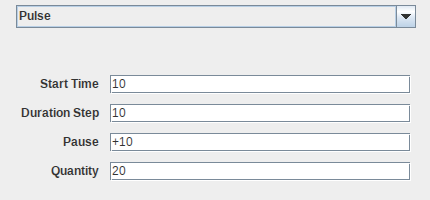
\includegraphics[scale=0.7]{condiguracao-carga-modulada3.png}
		\caption{Configuração para modular a carga como uma onda quadrada}
		\label{fig:condiguracao-carga-modulada3}
	\end{subfigure}\\[1ex]
	\begin{subfigure}{\linewidth}
		\centering
		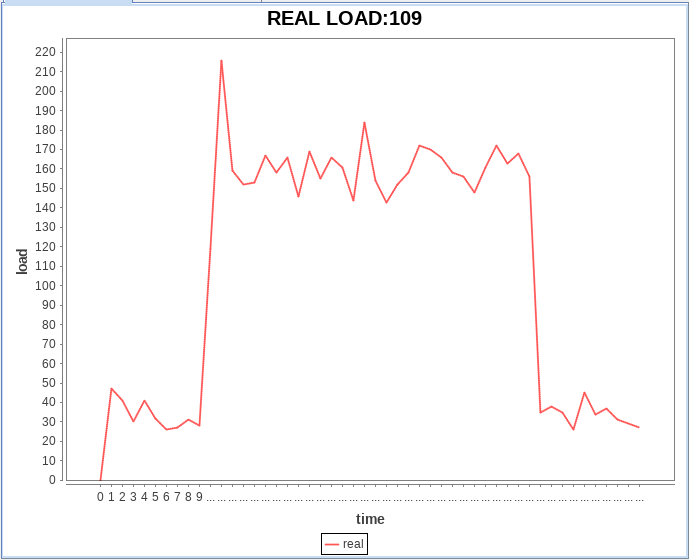
\includegraphics[scale=0.6]{grafico-carga-modulada3.png}
		\caption{Carga gerada com base nas configuração}
		\label{fig:grafico-carga-modulada3}
	\end{subfigure}
	\caption{Carga gerada com base na configuração: Onda Quadrada}
	\label{fig:carga-modulada3}
	\fautor
\end{figure}

Na figura \ref{fig:carga-modulada3} apresenta o resultado a modulação de uma onda quadrada, os parâmetros iniciais do Bench4Q referente a figura \ref{fig:condiguracao-carga-bench4q3} são os mesmos valores dos outros dois exemplos anteriores. Para gerar uma carga modula com comportamento oscilatório como a de uma onda quadrada, os parâmetros \ref{fig:condiguracao-carga-modulada3} são definidos com 10 segundos para \textit{Start Time}, 10 segundo de duração para \textit{Duration Step} e 10 para o \textit{Pause}, também configurado com 20 EBs. Para este exemplo vale salientar que para modular a carga como uma onda quadrada são dois parâmetros são importante e fundamentais \textit{Duration Step} e \textit{Pause}, estes devem ter os mesmos valores, pois eles é o quem manterão durante o período definido a carga em níveis baixo e máximo. 

%3º  - mostrar a analise e o impacto do carga de trabalho no sistema  
%Podemos agora usar os resultados da análise de desempenho para atender as metas estabelecidas no ponto 6.3.1. Por meio do modelo de QPN desenvolvido, que foram capazes de prever o desempenho do sistema em condições de funcionamento normais com 4 e 6 servidores WebLogic. Descobriu-se que usando o balanceador de carga original, seis nós de servidor de aplicação não foram suficientes para garantir tempos médios de resposta de transações de negócios abaixo de meio segundo. Atualizando o balanceador de carga com um CPU ligeiramente mais rápido levou à utilização de CPU do dropping balanceador de carga por um bom 20 por cento.
%Como resultado, os tempos de resposta de transações de concessionários melhorou em 15 a 27 por cento, encontrando o "meio segundo" exigência. No entanto, o aumento da intensidade da carga de trabalho além das condições de pico revelou que o balanceador de carga foi um recurso gargalo, impedindo-nos para escalar o sistema adicionando servidores WebLogic adicionais (veja a Figura 6.14). Assim, à luz do crescimento da carga de trabalho que o esperado, a empresa deve substituir a máquina balanceador de carga com um mais rápido ou considerar o uso de um método de balanceamento de carga mais eficiente. Depois de feito isso, a análise de desempenho deve ser repetida com o novo balanceador de carga para se certificar de que não há nenhum outro gargalos do sistema. Também deve ser assegurado que o balanceador de carga é configurado com threads suficientes para que não há contenção de discussão.
%Neste capítulo, a prática metodologia de modelagem de desempenho para DCS foi apresentada.
%A metodologia aproveita o poder de modelagem e expressividade do formalismo de modelagem QPN para melhorar a representatividade do modelo e permitir a previsão de desempenho precisas. Foi apresentado um estudo de caso detalhado no qual um modelo de um DCS realista foi construído e usado para analisar o seu desempenho e escalabilidade.
%O modelo de representatividade foi validado comparando suas previsões contra medições no sistema real. Foram considerados Um número de diferentes configurações de implantação e cenários de carga de trabalho. Além disso a CPU e I / O de contenção, demonstrou-se como alguns aspectos mais complexas do comportamento do sistema, tais como a contenção de rosca e processamento assíncrono, pode ser modelado. O modelo mostrou para refletir com precisão as características do sistema de desempenho e escalabilidade em estudo. O erro de modelagem para o tempo de resposta da transação não ultrapassou 21,2% e foi muito menor para a transferência de transações e utilização de recursos. A metodologia de modelagem de desempenho proposto fornece uma ferramenta poderosa para a engenharia de DCS desempenho.

%As análises apresentadas nessa Seção consideram a execução de rajadas de requisições dos usuários com e sem a presença de mecanismos de segurança, seguindo o planejamento definido na Seção anterior. Dessa forma, para uma melhor abordagem dos dados analisados, as avaliações foram divididas em duas Seções de acordo com o cenário.

\section{Contribuição}
\begin{frame}{Ilustração do impacto da modulação}
	Com a possibilidade da modulação de carga, é possível verificar o impacto da carga modulada no ambiente projetado para o trabalho de \cite{Edwin2015}.
\end{frame}
	
\begin{frame}{Ambiente Computacional do experimento}
	\begin{columns}
		\column{0.4\textwidth}
		\begin{minipage}[c][0.4\textheight][c]{\linewidth}
			\centering
			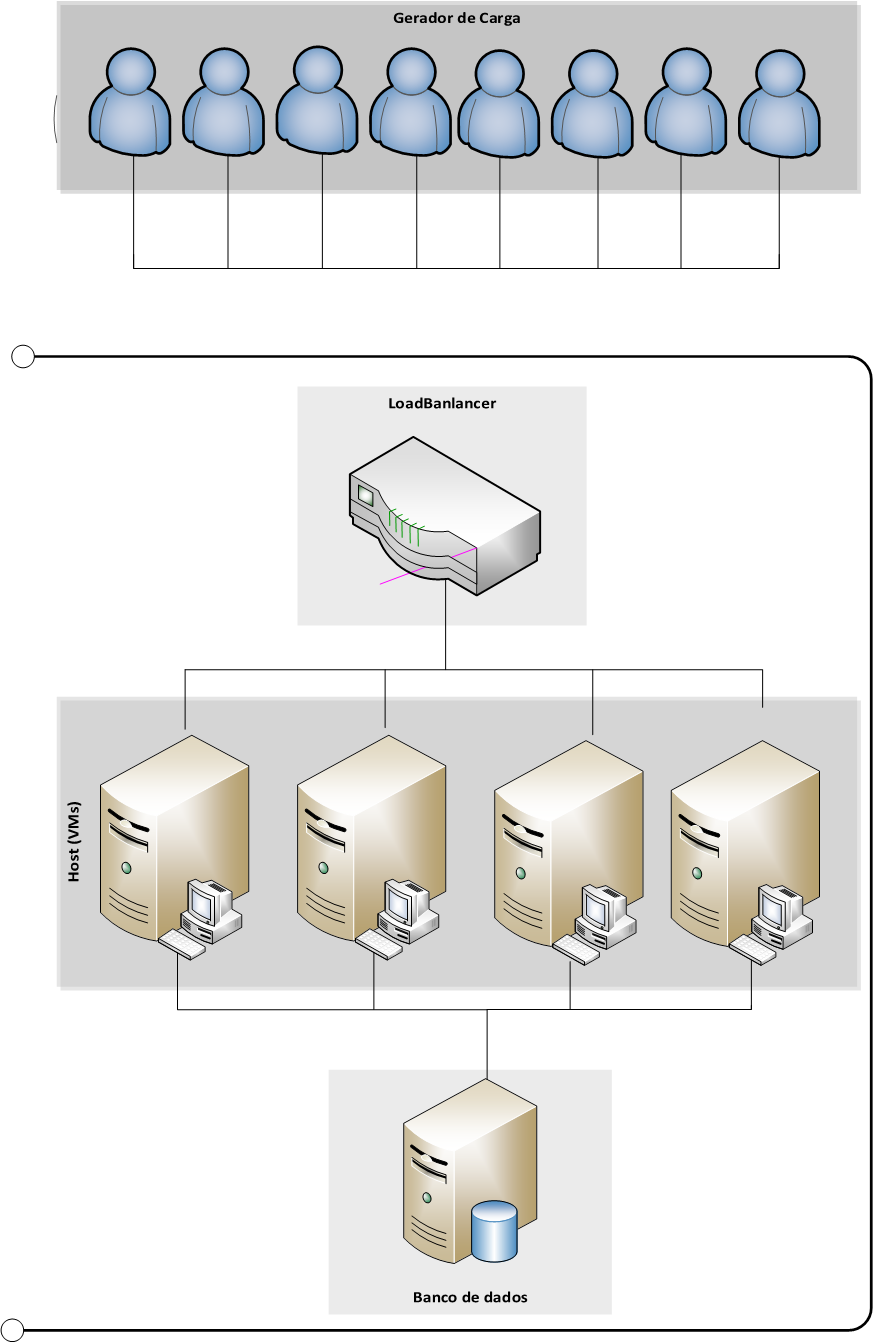
\includegraphics[scale=0.17]{../monograph/images/arquitetura-experimento.png}		
		\end{minipage}
		\column{0.6\textwidth}
		\begin{minipage}[c][0.4\textheight][c]{\linewidth}
			\begin{itemize}
				\item Gerador de Carga (\textit{Workload})
				\item Balanceador de carga (\textit{Load Balancer})
				\item Servidor Físico (\textit{Hypervisor})
				\item Servidor de dados (\textit{Data base})
			\end{itemize}
			\begin{figure}
				\centering
				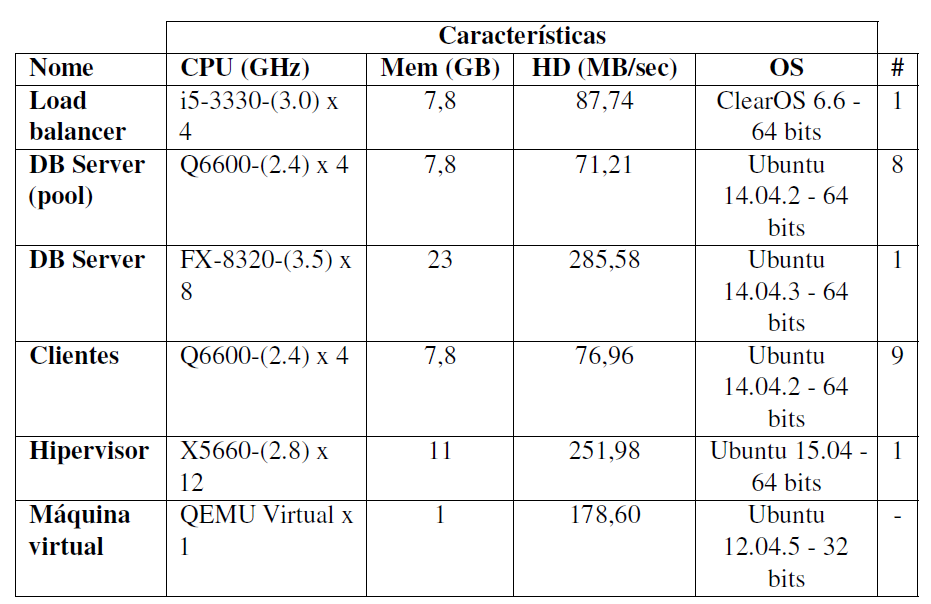
\includegraphics[scale=0.25]{images/soft-hard.png}
			\end{figure}
		\end{minipage}		
	\end{columns}
	
\end{frame}

%\begin{frame}{Elementos utilizados nos experimentos}
%	\begin{itemize}
%		\item Instalações do LaSDPC;
%		\item Foram utilizados dois \textit{clusters}.
%	\end{itemize}
%	\begin{figure}
%		\centering
%		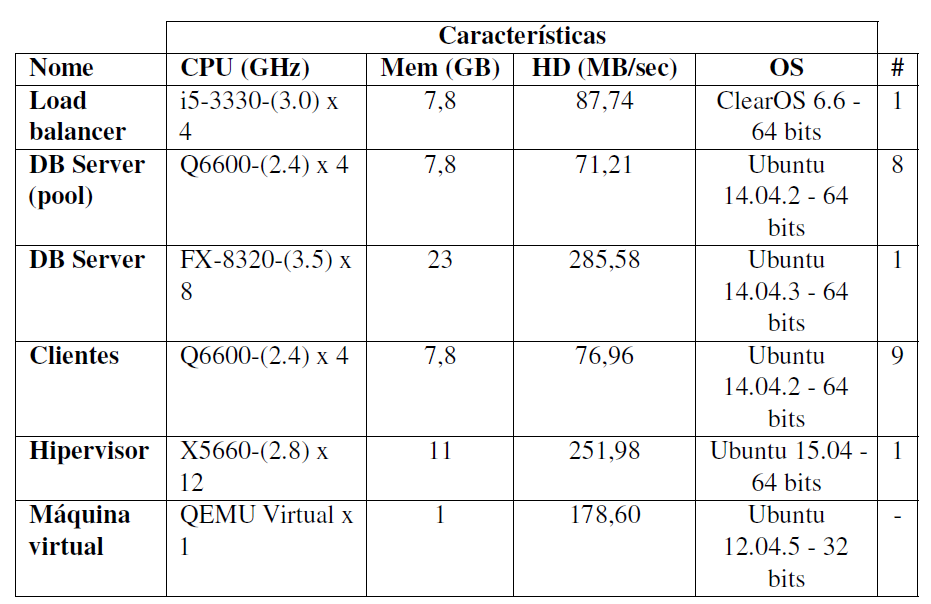
\includegraphics[width=0.6\textwidth]{images/soft-hard.png}
%		\caption{\textit{Hardware} e \textit{software} utilizados nos experimentos.}
%		\label{fig:table}
%	\end{figure}
%\end{frame}

\begin{frame}{Planejamento do experimento}
	\begin{columns}
		\column{0.5\textwidth}
		\begin{minipage}[c][0.4\textheight][c]{\linewidth}
			\centering
			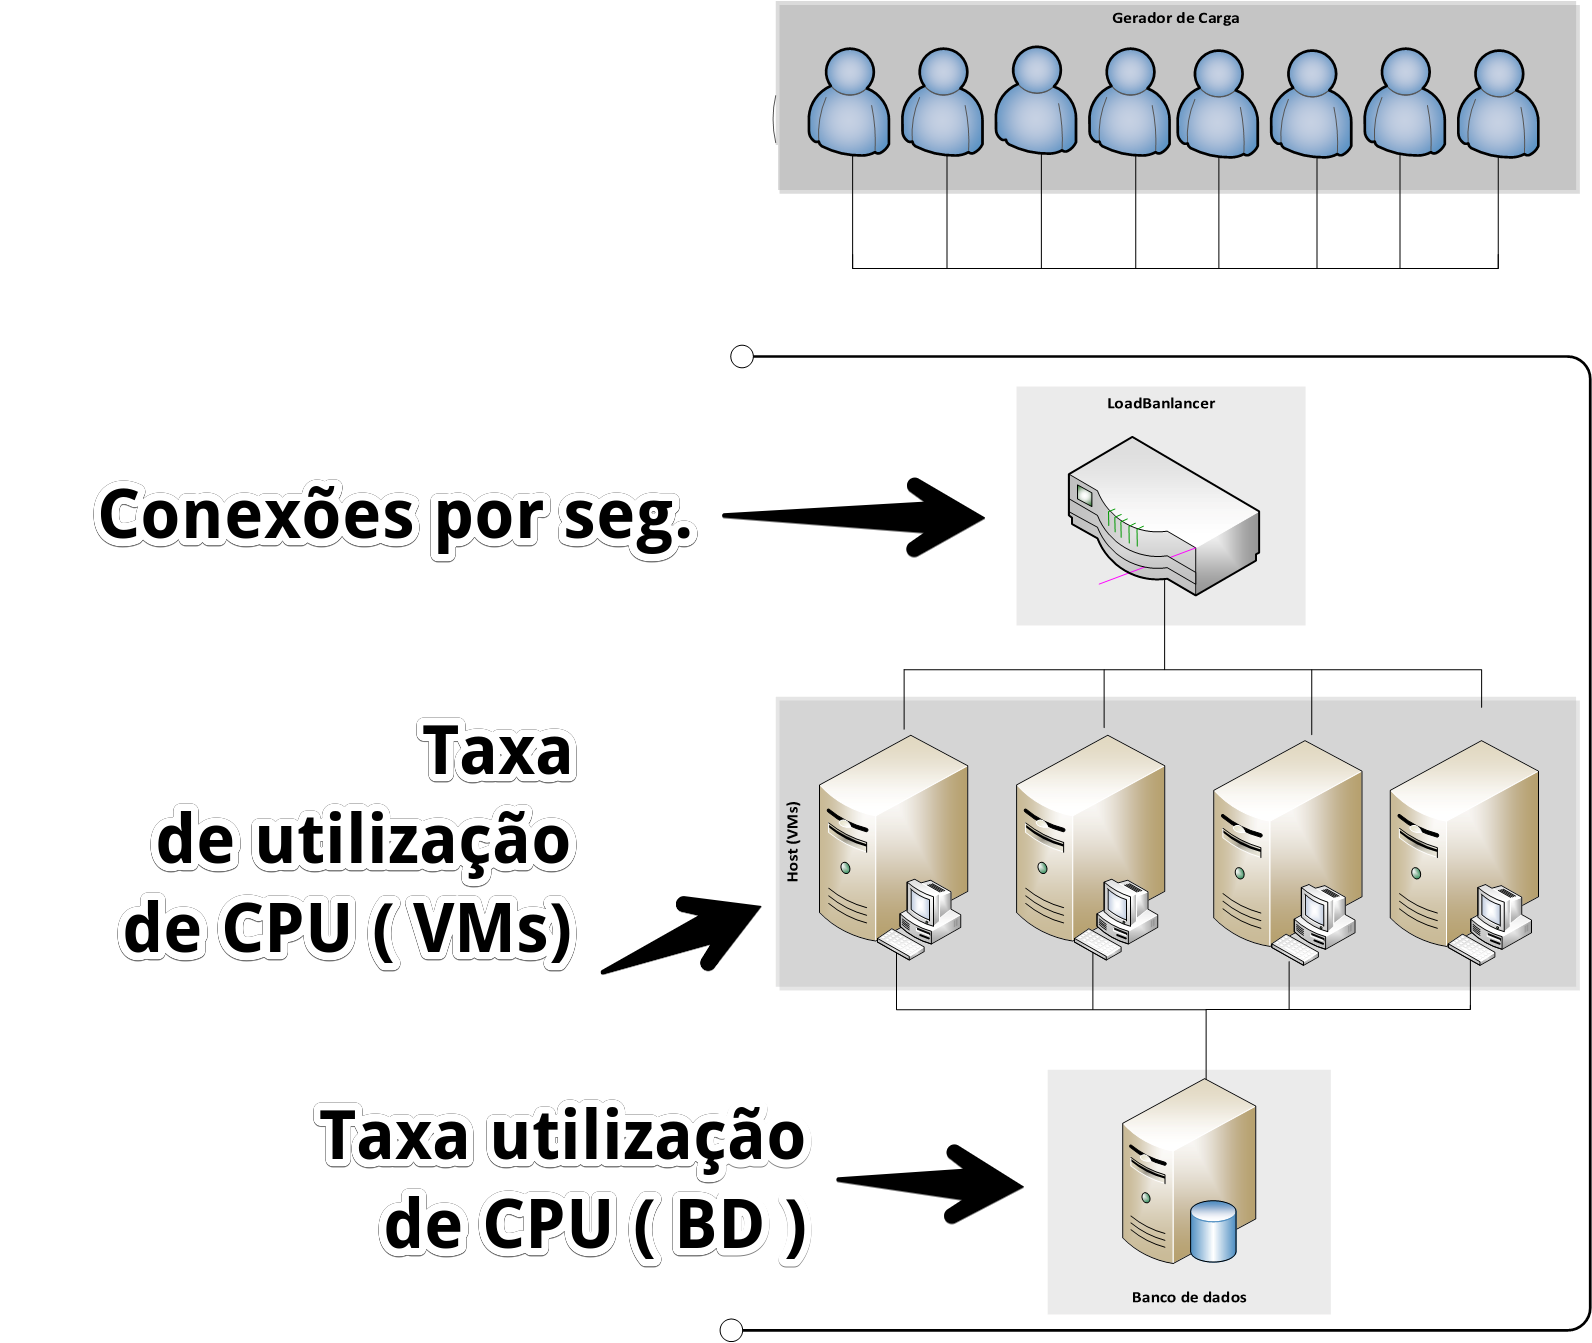
\includegraphics[scale=0.15]{images/metricas-arquitetura-experimento2.png}		
		\end{minipage}
		\column{0.5\textwidth}
		\begin{minipage}[c][0.4\textheight][c]{\linewidth}
			\begin{itemize}
				\item Carga inicial: (10 EBs)
				\item Carga reservada: (20 EBs)
			\end{itemize}
			\begin{figure}
				\centering
				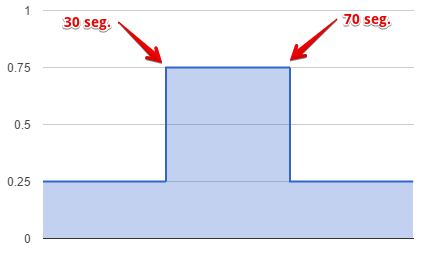
\includegraphics[scale=0.5]{images/carga-modulada-experimento.png}
			\end{figure}
			
		\end{minipage}		
	\end{columns}
	
\end{frame}

%\begin{frame}{Métrica transiente}
%	\begin{itemize}
%		\item \textbf{Conexões por segundo (\textit{Load Balancer}):} Conforme sugerido por \cite{Binnig2009}, medir a escalabilidade através do aumento dos interações web emitidos por segundo ao longo do tempo e de forma contínua contando a interação web que são respondidas em um intervalo de tempo de resposta,
%		
%		\item \textbf{Tempo de resposta (\textit{browsers}):} \cite{helder2014}, em um sistema dinâmico, cuja transformação entrada-saída não ocorre em tempo zero, mas é sujeita a uma inércia advinda dos processos físicos associados, possuí uma inércia intrínseca que atrasa o efeito que uma entrada terá na saída. Esses efeitos refletem no consequentemente nos comportamentos diversos que incluem retardo no tempo de resposta e possíveis oscilações; 	
%		
%	\end{itemize}
%\end{frame}
%
%\begin{frame}{Métrica transiente}
%	\begin{itemize}
%		\item \textbf{Taxa de utilização da CPU (VMs):} \cite{Nobile2013} afirma que diversas métricas podem ser analisadas para verificar o desempenho das máquinas virtuais, e cita alguns exemplos, como o tempo de inicialização, a taxa de utilização de CPU, o tempo médio de resposta e o \textit{throughput}, e usualmente, número de máquinas virtuais que hospedam serviços de interesse ao cliente e que respondem a uma carga de trabalho imposta por usuários através de requisições;
%		
%		\item \textbf{Taxa de utilização da CPU:} O trabalho apresentado por \cite{wang2009}, que lida com uma carga de trabalho variante no tempo e intensiva, demonstra que a CPU e I/O podem ser utilizadas para prever as necessidades dos recursos de um banco de dados e para orientar a alocação de recursos \textit{on-demand} de acordo com a exigência de carga de trabalho. Entretanto iremos somente considerar em nossos experimento a taxa de utilização do banco de dados.
%	\end{itemize}
%\end{frame}

%\begin{frame}{Resultados experimento}
%Com a possibilidade da modulação de carga, é possível verificar o impacto da carga modulada no ambiente projetado para o trabalho de \cite{Edwin2015}. 
%	\begin{itemize}
%		\item inicialmente utilizado 40\% da carga até o instante de 30 segundos de experimentação
%	
%		\item a partir de 30 segundos um crescimento brusco na carga utilizando os 60\% restante da carga, e gerando um degrau positivo. A carga mantém-se máxima, em 100\%, durante 40 segundos 
%	
%		\item apos decorridos 70 segundo de experimentação), a uma queda súbita voltando a trabalhar com 40\% da carga até o final do experimento.
%	\end{itemize}
%\end{frame}

%\begin{frame}{Conexões por segundo vs Tempo de resposta}
%	\begin{figure}[htb]
%		\centering
%		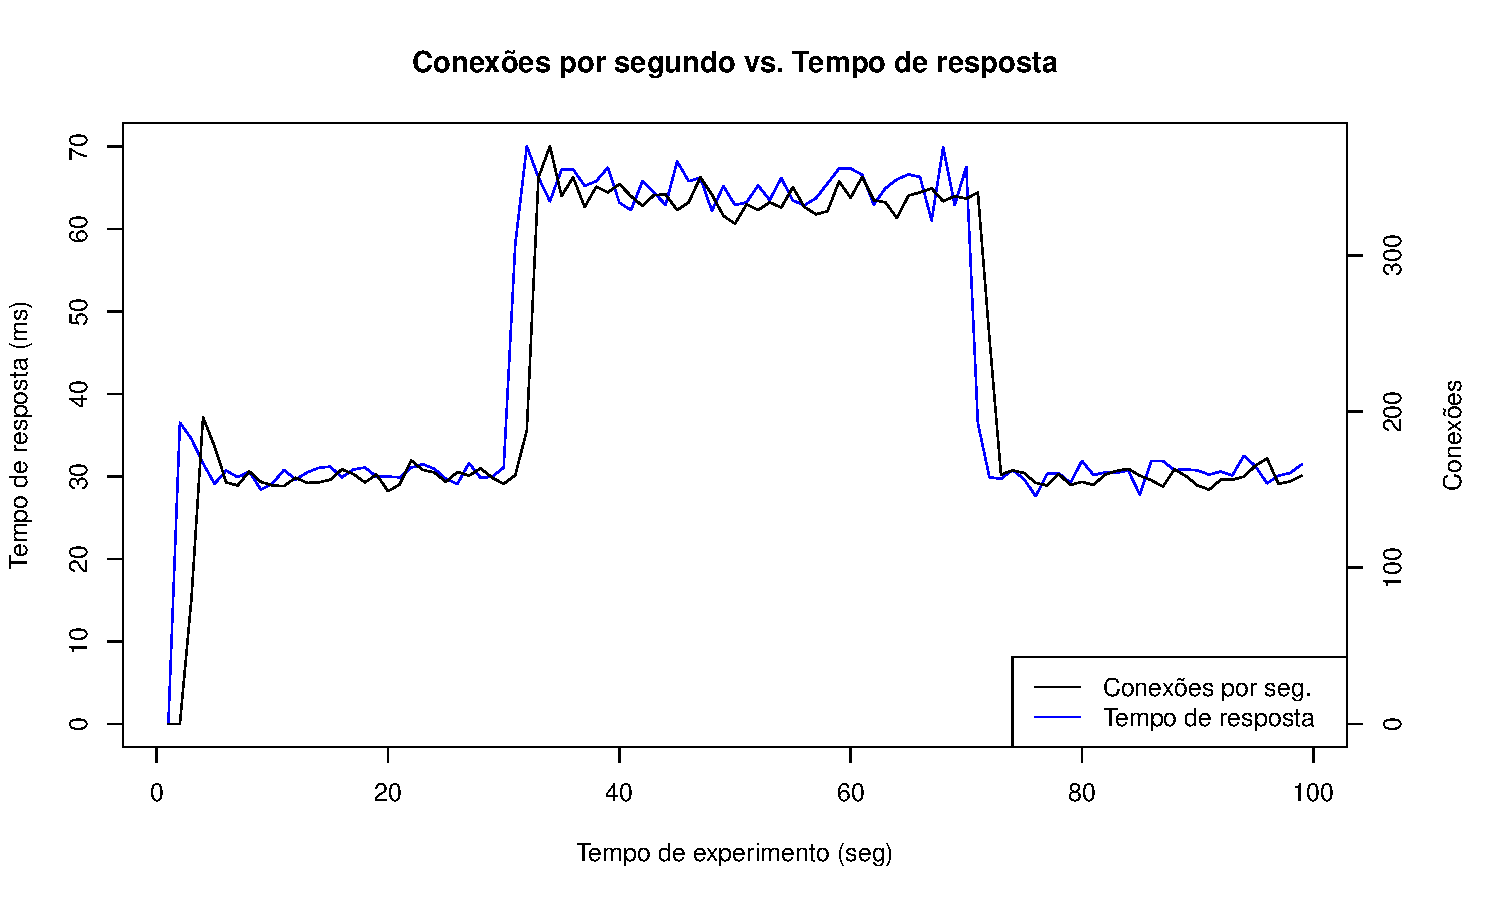
\includegraphics[scale=0.5]{../monograph/images/cps-resp60.pdf}	
%		\label{fig:cps-resp60}
%	\end{figure}
%\end{frame}

\begin{frame}{Conexões por segundo \& Média de utilização das CPU VMs}
	\begin{figure}[htb]
		\centering
		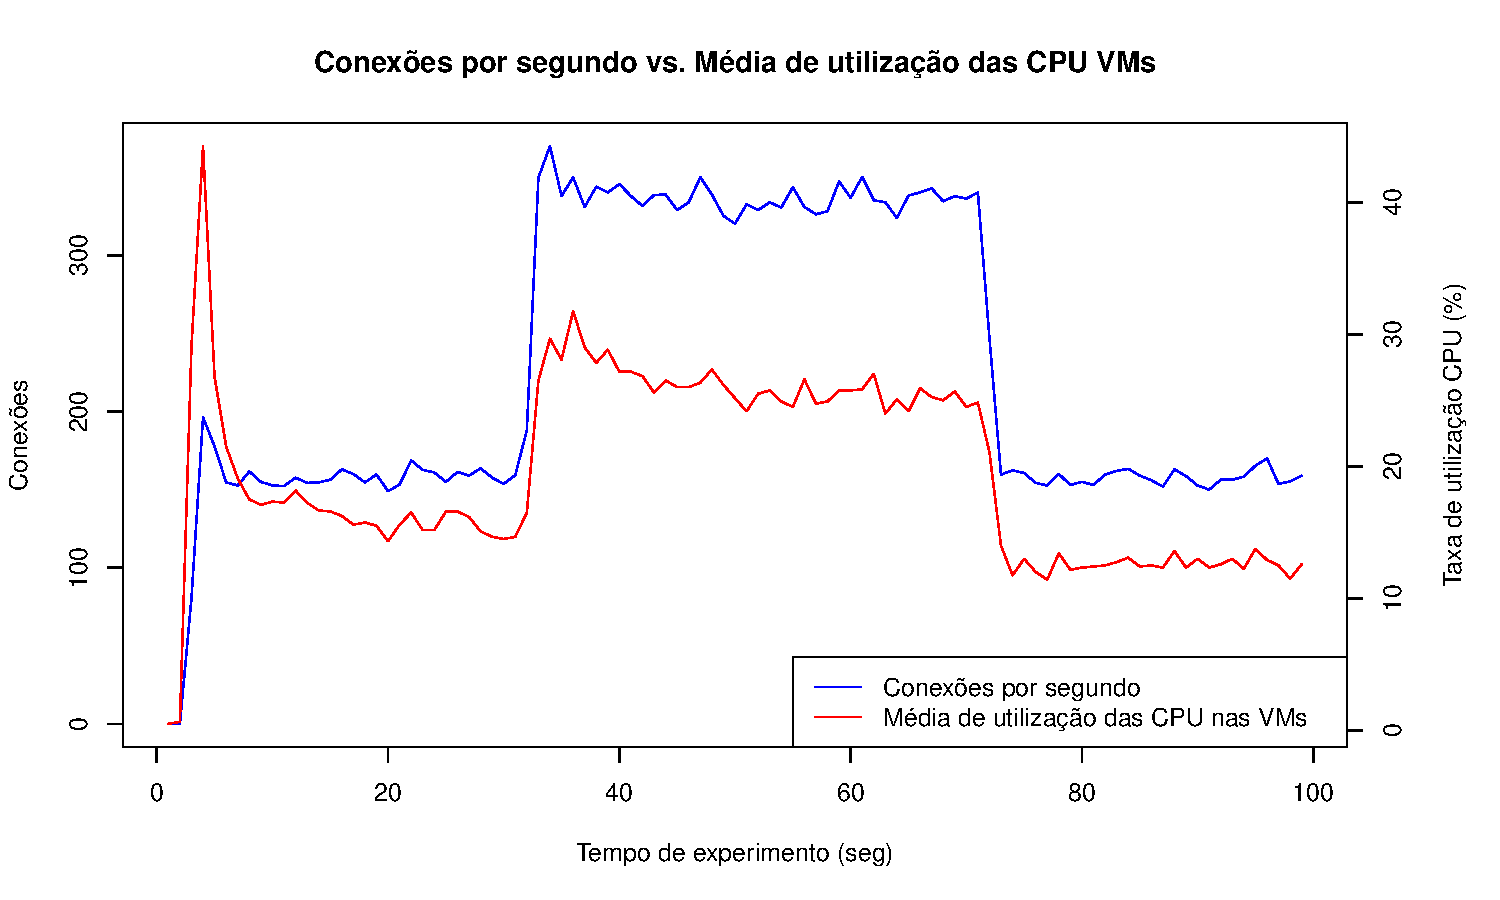
\includegraphics[scale=0.45]{../monograph/images/cps-vmcpu60.pdf}
		\label{fig:cps-vmcpu60}
	\end{figure}
\end{frame}

\begin{frame}{Conexões por segundo \& Utilização de CPU Banco de dados}
	\begin{figure}[htb]
		\centering
		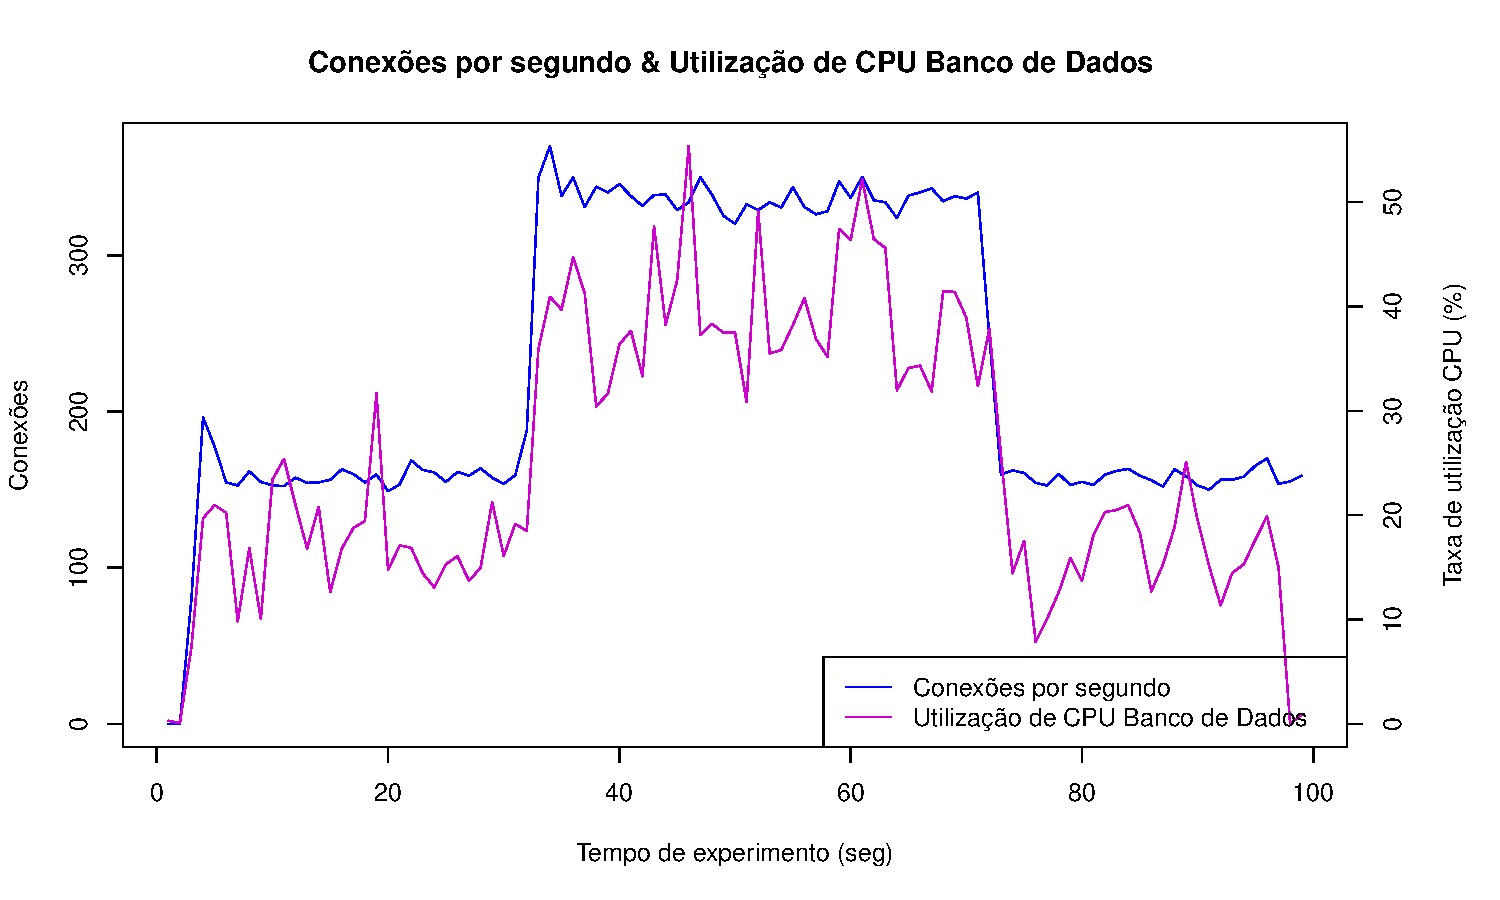
\includegraphics[scale=0.45]{../monograph/images/cps-dbcpu60.pdf}
		\label{fig:cps-dbcpu60}
	\end{figure}
\end{frame}

%\begin{frame}{Tempo de resposta \& Utilização de CPU Banco de dados}
%	\begin{figure}[htb]
%		\centering
%		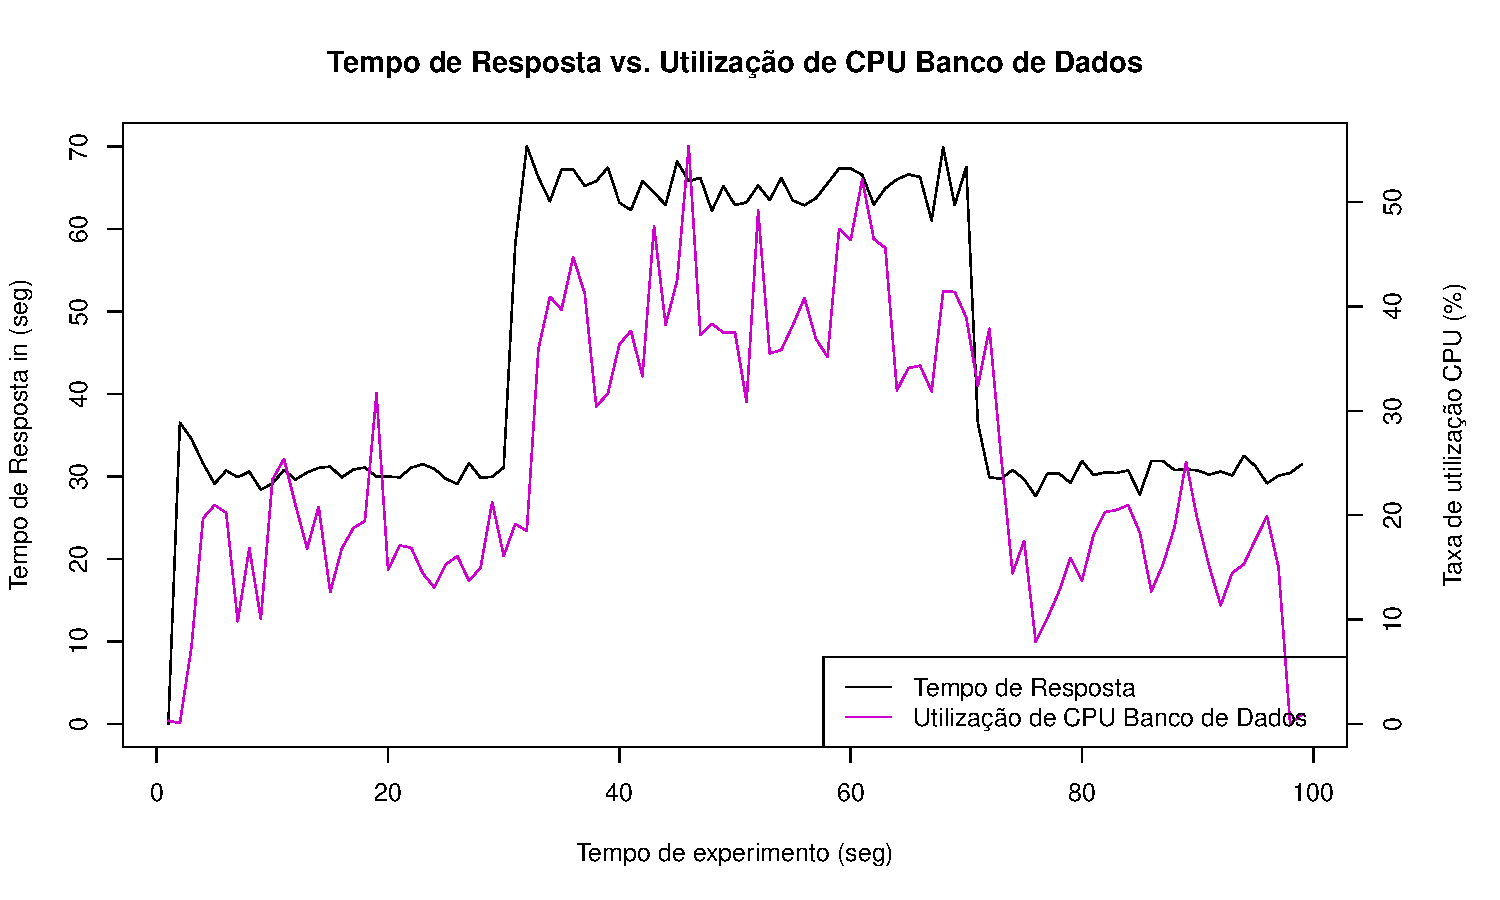
\includegraphics[scale=0.45]{../monograph/images/resp-dbcpu60.pdf}
%		\label{fig:resp-dbcpu60}
%	\end{figure}
%\end{frame}

\begin{frame}{Comparação PostgreSQL e DB2}
	\begin{columns}
		\begin{column}{0.5\textwidth}
			\begin{figure}
				\centering
				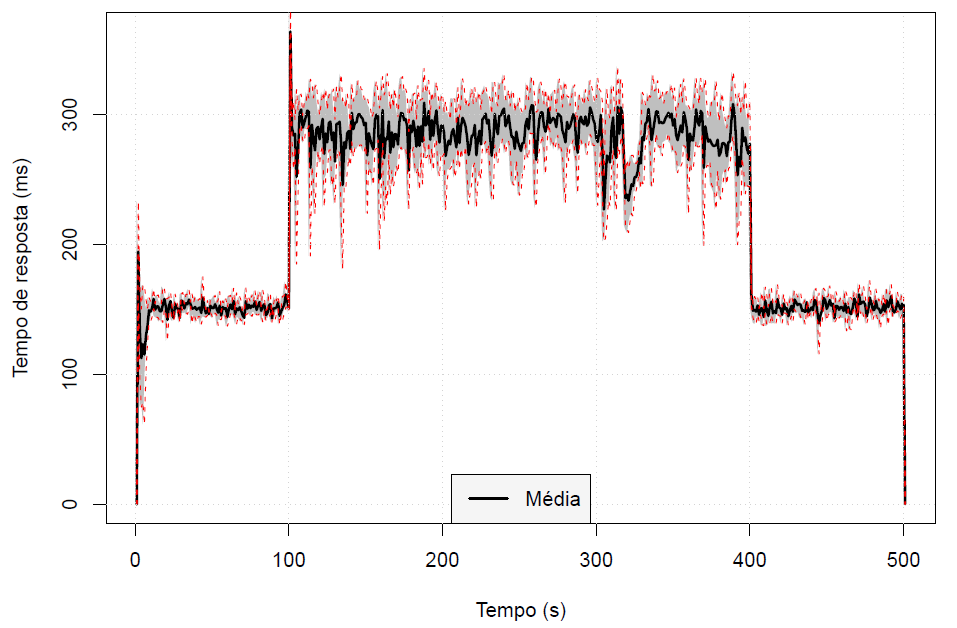
\includegraphics[width=0.9\textwidth]{images/tempo-resposta-postgres-crop.png}
			\end{figure}
			
		\end{column}
		
		\begin{column}{0.5\textwidth}
				\begin{figure}
					\centering
					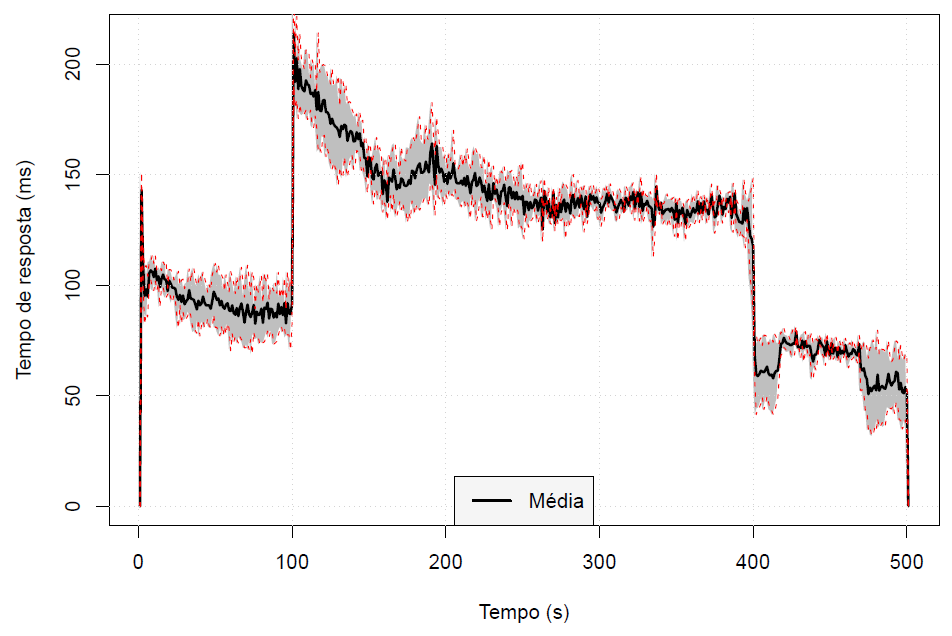
\includegraphics[width=0.9\textwidth]{images/tempo-resposta-db2-crop.png}
				\end{figure}
			
		\end{column}
	\end{columns}
	
	\caption{Resultados trabalho \cite{Edwin2015}}
\end{frame}


\begin{frame}{Utilização da metodologia de avaliação de desempenho não-estacionário}
	\begin{columns}
		\column{0.6\textwidth}
		\begin{figure}[htb]
			\centering
			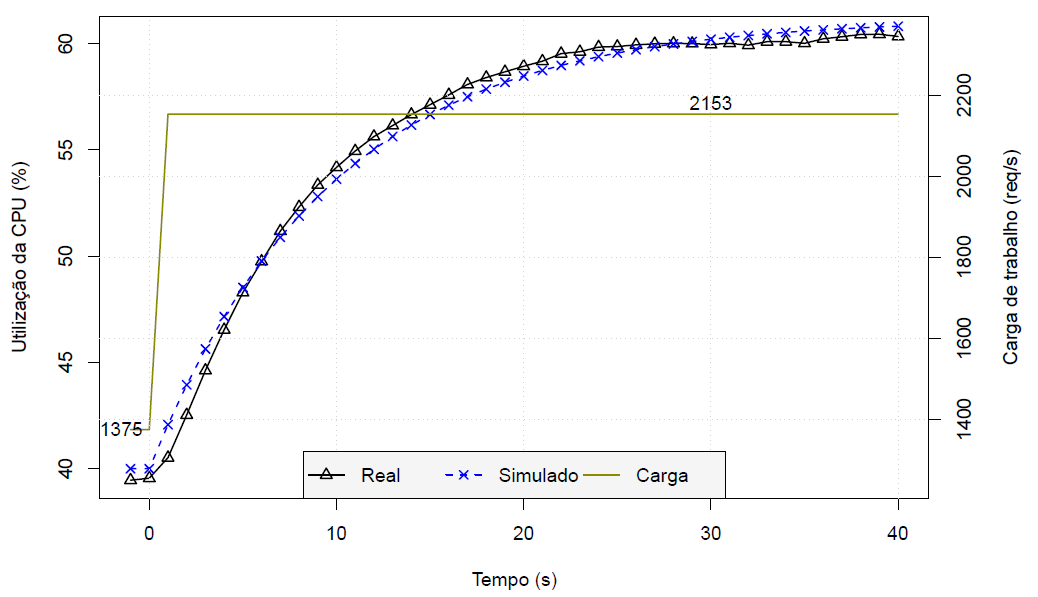
\includegraphics[scale=0.25]{images/resultado_edwin_identificao_sys.png}				
		\end{figure}
		\column{0.4\textwidth}
		\begin{block}{Domínio na frequência}
			\begin{equation}
				\small
				G(z) = \frac{b}{z - a}
			\end{equation}			
			\begin{equation}
				\small
				G(z) = \frac{0.002682}{z - 0.9057}
			\end{equation}							
		\end{block}
		\caption{Resultados trabalho \cite{Edwin2015}}				
				
	\end{columns}
	\begin{block}{Domínio no tempo}
		\begin{equation}
			\small	
			y(k) = -ay(k-1) + bu(k-1)
		\end{equation}			
		\begin{equation}
			\small
			y(k) = -0.9057y(k-1) + 0.002682u(k-1)
		\end{equation}
	\end{block}

\end{frame}







%==================== Conclusao
\section{Conclusão}
A computação em nuvem popularizou um serviço de comercialização se de capacidade computacional na qual a infraestrutura, plataforma ou \textit{software} são ofertados como produto sob demanda e onde os recursos são elásticos, despertando o interesse tanto da comunidade acadêmica quanto da indústria. Atualmente a maioria das grandes soluções de sistemas computacionais são compostas por \textit{mult-tiers}, inclusive quando se refere a aplicações web, devido à flexibilidade de escalabilidade. Para essas aplicações, o planejamento de capacidade é um requisito crítico para determinar a quantidade de recursos exigido para garantia de QoS. No entanto, o planejamento de capacidade é usualmente uma decisão de longo prazo em que, e os recursos são determinados por critérios estáticos. Desta forma, os recursos podem revelar uma sobrecarga em situações de perturbação, mesmo que os níveis de QoS esteja dentro da faixa aceitável para a carga estacionária. %Isso ocorre, devido a utilização da avaliação de desempenho, que é comumente destinada a responder a perguntas estáticas como qual o limite do sistema mediante a uma carga estacionaria imposta. 

Em sistemas que apresentam dinâmica acentuada, a avaliação de desempenho deve considerar que os períodos de regime transiente são importantes. Junto aos mecanismos de elasticidade dos recursos sob demanda, vem a necessidade do autogerenciamento dos recursos. Existem vários trabalhos disponíveis na literatura que lidam e tratam da gestão dos recursos computacionais. Neste trabalho há interesse na modelagem do sistema na forma de uma representação analítica capaz de reproduzir o comportamento dinâmico do sistema, onde o período transiente tem grande colaboração e impacto na política de gerenciamento dos recursos. Um diferencial em relação as abordagens convencionais o objetivo de determinar como a capacidade do sistema em lidar com a variação da carga de trabalho, ao invés de, o desempenho apenas com a carga de trabalho estacionaria.

Mediante a uma arquitetura conceitual proposta por \citeonline{Lourenco2015} e \citeonline{Edwin2015} propõe uma metodologia que descreve e especifica os passos para modelar um sistema computacional por meio de um \textit{benchmark}. No entanto, não foram encontrados \textit{benchmarks} que estimulem a dinâmica do sistema e que permitem uma avaliação em regime transiente, bem como não foram identificados \textit{benchmarks} que sigam a especificação de requisitos proposta por \citeonline{Lourenco2015}.
Este trabalho apresentou uma extensão de um \textit{benchmark}, o Bench4Q, capaz de modelar a sua carga de trabalho de tal maneira a estimular o sistema a apresentar sua dinâmica através da carga. Essa extensão segue um dos requisitos MESC, o modulo \textit{Demand}, proposto por \citeonline{Lourenco2015}, que se restringe a modulação da carga de trabalho, acrescendo-a de provisões para gerar perturbações programadas. Essa extensão, obedece ao padrão de implementação e usabilidade nativas do \textit{benchmark} Bench4Q. A extensão é provida de uma interface gráfica que possibilita a modelagem da carga através da inserção de parâmetros.

Para atingir o objetivo proposto, foi necessária a alteração da carga de trabalho nativa do Bench4Q. Essa modificação resultou na modulação da carga, possibilitando a geração de Degrau Positivo com a carga. Este modelo de carga tem como característica a alteração da sua potência de maneira brusca e repentina. Também é possível gerar um Degrau Negativo que tem efeito oposto ao Degrau Positivo, ou seja, o modelo da carga tem por característica a queda repentina de sua potência. Outra modelagem de carga que a extensão permite é a geração de uma Onda Quadrada, onde existe uma alternância entre os dois modelos descritos anteriormente. 
Por se tratar de um trabalho de extensão de \textit{benchmark} difundido e grande complexidade, as alterações efetuadas trouxeram dificuldades relacionadas a implementação. A falta de uma documentação técnica gerou grande esforço no entendimento e compreensão da implementação original, necessitando muitas vezes a depuração do código para o claro entendimento do seu fluxo de funcionamento tão quando os módulos envolvidos.

O projeto apresentou exemplos práticos das modelagem das cargas propostas (Degrau Positivo, Degrau Negativo e Onda Quadrada) através dos resultados gerados pelo próprio \textit{benchmark}. Os resultados da presente pesquisa foram adequado, na medida em que responderam positivamente ao objetivo do trabalho. O trabalho contemplou uma bateria de experimentos práticos em um ambiente controlado \textit{mult-tier}. Na execução das fases de experimentos, foi elaborado o planejamento do experimento, a coleta de dados e juntamente a análises dos resultados obtidos, resultando em um conjunto de contribuições para a área de pesquisa:
\begin{itemize}
	\item A elaboração de uma documentação padronizada da mesma forma que a original do Bench4Q, contando com versão em inglês que se encontra no apêndice \ref{chapter:documentacao};
	
	\item Impacto da carga modulada: mediante a modulação da carga através da extensão, é possível excitar o sistema a apresentar a sua dinâmica, contribuindo para trabalhos que tem por necessidade a modelagem do sistema e do seu comportamento dinâmico;
	
	\item Dinâmica entre camadas: ao se tratar de um sistema de multicamadas, foi possível perceber, juntamente com a modulação da carga, a dinâmica intrínseca entre as camadas do sistema. Os efeitos combinados de atrasos intrínsecos, ainda que pequenos, e sua propagação por todo as camadas interligados geraram um comportamento dinâmico significante e apreciável;
	
	\item Métrica que mascara: por consequência da dinâmica inerente ao sistema multicamadas, foi possível vislumbrar que nem toda métrica apresenta a realidade quando se lida com um sistema multicamadas. Neste trabalho, foi possível observar esse fato na métrica tempo de resposta.
\end{itemize} 

O presente trabalho foi desenvolvido em consequência aos interesse de estudo da pesquisa de \citeonline{Edwin2015}, e em paralelo a outra iniciativa de \citeonline{Lourenco2015} que especificam a identificação de capacidade dinâmica em sistemas computacionais e como tratá-las com técnicas de modelagem de sistemas. Os resultados do presente trabalho contribuem para ambos os projetos com a disponibilização de um \textit{benchmark} que auxilia na modelagem de sistemas computacionais dinâmicos.

\section{Trabalhos Futuros}
O presente trabalho de mestrado contribuiu para o desenvolvimento de técnicas e estudos interessados na dinâmica do sistema. Todavia, existe uma gama de trilhas a serem exploradas até que a importância da dinâmica de sistemas computacionais tenha maior apreço, como nos casos das ciências e engenharias. Consequentemente este trabalho não finaliza as possibilidades de estudo relacionadas e outros estudos podem ser desenvolvidos a partir dos resultados e constatações identificadas dentre os são:
\begin{itemize}
	\item \textbf{Novas formas de pertubação:} com base nas proposta de \cite{Hellerstein2004} existem outras funções que auxiliam a excitar o sistema a apresentarem a sua dinâmica. 
	
	\item \textbf{Avaliação da dinâmica em sistemas multicamadas:} com o presente trabalho, foi possível observar a dinâmica entre as camadas do sistema, entretanto o presente trabalho não cobre com um planejamento de experimentos utilizando métodos estatísticos por meio de avaliações de desempenho
	
	\item \textbf{Avaliação de métricas de planejamento de recursos em ambiente multicamadas:} este trabalho também revelou que existem métricas que podem mascarar a realidade, neste contexto é importante uma análise das principais métricas de diferentes técnicas para o planejamento de recursos sob um ambiente de multicamadas
\end{itemize} 	


\begin{frame}
    \begin{center}
        \textbf{Obrigado!}
    \end{center}   
\end{frame}

%==================== Exemplos
%=\section{Exemplos}
%\begin{frame}
	\frametitle{Sample frame title}
	This is a text in second frame. 
	For the sake of showing an example.
	
	\begin{itemize}
		\item<1-> Text visible on slide 1
		\item<2-> Text visible on slide 2
		\item<3> Text visible on slide 3
		\item<4-> Text visible on slide 4
	\end{itemize}
	
\end{frame}

\begin{slide}{Slide Title}
	You can see a list of items below. \pause \\
	There are commands to make them appear sequentially
	\begin{itemize}[type=1]
		\item<2> This is an item
		\item<3> Second item
		\item<4> Third item
	\end{itemize}
\end{slide}

\begin{frame}
	\frametitle{Sample frame title}
 
	In this slide, some important text will be \alert{highlighted} beause it's important. Please, don't abuse it.
 
	\begin{block}{Remark}
		Sample text
	\end{block}
	 
	\begin{alertblock}{Important theorem}
		Sample text in red box
	\end{alertblock}
 
	\begin{examples}
		Sample text in green box. "Examples" is fixed as block title.
	\end{examples}
\end{frame}

\begin{frame}
	\frametitle{Two-column slide}
	
	\begin{columns}
		
		\column{0.5\textwidth}
		This is a text in first column.
		$$E=mc^2$$
		\begin{itemize}
			\item First item
			\item Second item
		\end{itemize}
		
		\column{0.5\textwidth}
		This text will be in the second column
		and on a second tought this is a nice looking
		layout in some cases.
	\end{columns}
\end{frame}

\begin{frame}[fragile]\frametitle{Linguagem de programa\c c\~ao}
	Para mostrar c\'odigos de linguagem de programa\c c\~ao use o pacote \verb|minted|.
	
	Exemplo de c\'odigo Java.
	
	\begin{javacode}
		public class HelloWorldApp {
			public static void main (String args[])
			{
				System.out.println("Hello World!");
			}
		}
	\end{javacode}
	
	Para compilar com o pacote \verb|minted| \'e necess\'ario usar o comando \verb|-shell-escape| pelo terminal.
	
	\begin{minted}[bgcolor=lightgray!20]{bash}
		pdflatex -shell-escape minted01.tex
		ou
		latexmk -pdf -shell-escape minted01.tex
	\end{minted}
\end{frame}

\begin{frame}\frametitle{Inserindo figuras}
	Figuras devem ser inseridas no formato PNG, JPG ou PDF.
	
	\begin{figure}[h]
		\centering
		\includegraphics[height=0.6\paperheight]{figuras/figCoordEsf02}
		%\includegraphics[height=6cm]{figCoordEsf02}
		\caption{Sistema de coordenadas esf\'ericas.}\label{figCoordEsf02}
	\end{figure}
\end{frame}
Com o pacote TikZ podemos inserir figuras desenhadas em TikZ.
% Frame 10: figuras TikZ
\begin{frame}\frametitle{Figuras TikZ}
	Figuras feitas com TikZ.
	
	\begin{figure}[h]
		\centering
		\input{figuras/integral}
		\caption{Integral.}\label{figintegral}
	\end{figure}
\end{frame}

\begin{frame}\frametitle{Tabelas}
	\begin{table}
		\centering
		\begin{tabular}{cclrr}
			\toprule
			ID & Quant & Produto & Unit & Total\\
			\midrule
			1 & 2 & manga     & 3,00 & 6,00\\
			2 & 7 & laranja   & 1,20 & 8,40\\
			3 & 5 & banana    & 3,50 & 17,50\\
			4 & 3 & melancia  & 8,00 & 24,00\\
			5 & 4 & abacaxi   & 4,00 & 16,00\\
			\midrule
			Total &   &      &      & 71,90\\
			\bottomrule
		\end{tabular}
		\caption{Lista de compras}
	\end{table}
\end{frame}

\begin{frame}\frametitle{Transi\c c\~ao}
	Um pequeno exemplo de transi\c c\~ao.
	
	\pause
	
	\begin{enumerate}[a)]
		\item<2-< primeiro;
		\item<3-< segundo;
		\item<4-< terceiro.
	\end{enumerate}
\end{frame}

\begin{frame}\frametitle{Bibliografia}
	\bibliographystyle{icmc}
	\bibliography{content/bibliografia}
\end{frame}


\end{document}